%% bare_jrnl.tex
%% V1.4b
%% 2015/08/26
%% by Michael Shell
%% see http://www.michaelshell.org/
%% for current contact information.
%%
%% This is a skeleton file demonstrating the use of IEEEtran.cls
%% (requires IEEEtran.cls version 1.8b or later) with an IEEE
%% journal paper.
%%
%% Support sites:
%% http://www.michaelshell.org/tex/ieeetran/
%% http://www.ctan.org/pkg/ieeetran
%% and
%% http://www.ieee.org/

%%*************************************************************************
%% Legal Notice:
%% This code is offered as-is without any warranty either expressed or
%% implied; without even the implied warranty of MERCHANTABILITY or
%% FITNESS FOR A PARTICULAR PURPOSE! 
%% User assumes all risk.
%% In no event shall the IEEE or any contributor to this code be liable for
%% any damages or losses, including, but not limited to, incidental,
%% consequential, or any other damages, resulting from the use or misuse
%% of any information contained here.
%%
%% All comments are the opinions of their respective authors and are not
%% necessarily endorsed by the IEEE.
%%
%% This work is distributed under the LaTeX Project Public License (LPPL)
%% ( http://www.latex-project.org/ ) version 1.3, and may be freely used,
%% distributed and modified. A copy of the LPPL, version 1.3, is included
%% in the base LaTeX documentation of all distributions of LaTeX released
%% 2003/12/01 or later.
%% Retain all contribution notices and credits.
%% ** Modified files should be clearly indicated as such, including  **
%% ** renaming them and changing author support contact information. **
%%*************************************************************************


% *** Authors should verify (and, if needed, correct) their LaTeX system  ***
% *** with the testflow diagnostic prior to trusting their LaTeX platform ***
% *** with production work. The IEEE's font choices and paper sizes can   ***
% *** trigger bugs that do not appear when using other class files.       ***                          ***
% The testflow support page is at:
% http://www.michaelshell.org/tex/testflow/



\documentclass[journal]{IEEEtran}
%
% If IEEEtran.cls has not been installed into the LaTeX system files,
% manually specify the path to it like:
% \documentclass[journal]{../sty/IEEEtran}


\usepackage{graphicx}
\usepackage{algorithm}
\usepackage{algorithmicx}
\usepackage{algpseudocode}
\usepackage{amsmath}


% Some very useful LaTeX packages include:
% (uncomment the ones you want to load)


% *** MISC UTILITY PACKAGES ***
%
%\usepackage{ifpdf}
% Heiko Oberdiek's ifpdf.sty is very useful if you need conditional
% compilation based on whether the output is pdf or dvi.
% usage:
% \ifpdf
%   % pdf code
% \else
%   % dvi code
% \fi
% The latest version of ifpdf.sty can be obtained from:
% http://www.ctan.org/pkg/ifpdf
% Also, note that IEEEtran.cls V1.7 and later provides a builtin
% \ifCLASSINFOpdf conditional that works the same way.
% When switching from latex to pdflatex and vice-versa, the compiler may
% have to be run twice to clear warning/error messages.


% *** CITATION PACKAGES ***
%
%\usepackage{cite}
% cite.sty was written by Donald Arseneau
% V1.6 and later of IEEEtran pre-defines the format of the cite.sty package
% \cite{} output to follow that of the IEEE. Loading the cite package will
% result in citation numbers being automatically sorted and properly
% "compressed/ranged". e.g., [1], [9], [2], [7], [5], [6] without using
% cite.sty will become [1], [2], [5]--[7], [9] using cite.sty. cite.sty's
% \cite will automatically add leading space, if needed. Use cite.sty's
% noadjust option (cite.sty V3.8 and later) if you want to turn this off
% such as if a citation ever needs to be enclosed in parenthesis.
% cite.sty is already installed on most LaTeX systems. Be sure and use
% version 5.0 (2009-03-20) and later if using hyperref.sty.
% The latest version can be obtained at:
% http://www.ctan.org/pkg/cite
% The documentation is contained in the cite.sty file itself.


% *** GRAPHICS RELATED PACKAGES ***
%
\ifCLASSINFOpdf
% \usepackage[pdftex]{graphicx}
% declare the path(s) where your graphic files are
% \graphicspath{{../pdf/}{../jpeg/}}
% and their extensions so you won't have to specify these with
% every instance of \includegraphics
% \DeclareGraphicsExtensions{.pdf,.jpeg,.png}
\else
% or other class option (dvipsone, dvipdf, if not using dvips). graphicx
% will default to the driver specified in the system graphics.cfg if no
% driver is specified.
% \usepackage[dvips]{graphicx}
% declare the path(s) where your graphic files are
% \graphicspath{{../eps/}}
% and their extensions so you won't have to specify these with
% every instance of \includegraphics
% \DeclareGraphicsExtensions{.eps}
\fi
% graphicx was written by David Carlisle and Sebastian Rahtz. It is
% required if you want graphics, photos, etc. graphicx.sty is already
% installed on most LaTeX systems. The latest version and documentation
% can be obtained at: 
% http://www.ctan.org/pkg/graphicx
% Another good source of documentation is "Using Imported Graphics in
% LaTeX2e" by Keith Reckdahl which can be found at:
% http://www.ctan.org/pkg/epslatex
%
% latex, and pdflatex in dvi mode, support graphics in encapsulated
% postscript (.eps) format. pdflatex in pdf mode supports graphics
% in .pdf, .jpeg, .png and .mps (metapost) formats. Users should ensure
% that all non-photo figures use a vector format (.eps, .pdf, .mps) and
% not a bitmapped formats (.jpeg, .png). The IEEE frowns on bitmapped formats
% which can result in "jaggedy"/blurry rendering of lines and letters as
% well as large increases in file sizes.
%
% You can find documentation about the pdfTeX application at:
% http://www.tug.org/applications/pdftex


% *** MATH PACKAGES ***
%
%\usepackage{amsmath}
% A popular package from the American Mathematical Society that provides
% many useful and powerful commands for dealing with mathematics.
%
% Note that the amsmath package sets \interdisplaylinepenalty to 10000
% thus preventing page breaks from occurring within multiline equations. Use:
%\interdisplaylinepenalty=2500
% after loading amsmath to restore such page breaks as IEEEtran.cls normally
% does. amsmath.sty is already installed on most LaTeX systems. The latest
% version and documentation can be obtained at:
% http://www.ctan.org/pkg/amsmath


% *** SPECIALIZED LIST PACKAGES ***
%
%\usepackage{algorithmic}
% algorithmic.sty was written by Peter Williams and Rogerio Brito.
% This package provides an algorithmic environment fo describing algorithms.
% You can use the algorithmic environment in-text or within a figure
% environment to provide for a floating algorithm. Do NOT use the algorithm
% floating environment provided by algorithm.sty (by the same authors) or
% algorithm2e.sty (by Christophe Fiorio) as the IEEE does not use dedicated
% algorithm float types and packages that provide these will not provide
% correct IEEE style captions. The latest version and documentation of
% algorithmic.sty can be obtained at:
% http://www.ctan.org/pkg/algorithms
% Also of interest may be the (relatively newer and more customizable)
% algorithmicx.sty package by Szasz Janos:
% http://www.ctan.org/pkg/algorithmicx


% *** ALIGNMENT PACKAGES ***
%
%\usepackage{array}
% Frank Mittelbach's and David Carlisle's array.sty patches and improves
% the standard LaTeX2e array and tabular environments to provide better
% appearance and additional user controls. As the default LaTeX2e table
% generation code is lacking to the point of almost being broken with
% respect to the quality of the end results, all users are strongly
% advised to use an enhanced (at the very least that provided by array.sty)
% set of table tools. array.sty is already installed on most systems. The
% latest version and documentation can be obtained at:
% http://www.ctan.org/pkg/array


% IEEEtran contains the IEEEeqnarray family of commands that can be used to
% generate multiline equations as well as matrices, tables, etc., of high
% quality.


% *** SUBFIGURE PACKAGES ***
%\ifCLASSOPTIONcompsoc
%  \usepackage[caption=false,font=normalsize,labelfont=sf,textfont=sf]{subfig}
%\else
%  \usepackage[caption=false,font=footnotesize]{subfig}
%\fi
% subfig.sty, written by Steven Douglas Cochran, is the modern replacement
% for subfigure.sty, the latter of which is no longer maintained and is
% incompatible with some LaTeX packages including fixltx2e. However,
% subfig.sty requires and automatically loads Axel Sommerfeldt's caption.sty
% which will override IEEEtran.cls' handling of captions and this will result
% in non-IEEE style figure/table captions. To prevent this problem, be sure
% and invoke subfig.sty's "caption=false" package option (available since
% subfig.sty version 1.3, 2005/06/28) as this is will preserve IEEEtran.cls
% handling of captions.
% Note that the Computer Society format requires a larger sans serif font
% than the serif footnote size font used in traditional IEEE formatting
% and thus the need to invoke different subfig.sty package options depending
% on whether compsoc mode has been enabled.
%
% The latest version and documentation of subfig.sty can be obtained at:
% http://www.ctan.org/pkg/subfig


% *** FLOAT PACKAGES ***
%
%\usepackage{fixltx2e}
% fixltx2e, the successor to the earlier fix2col.sty, was written by
% Frank Mittelbach and David Carlisle. This package corrects a few problems
% in the LaTeX2e kernel, the most notable of which is that in current
% LaTeX2e releases, the ordering of single and double column floats is not
% guaranteed to be preserved. Thus, an unpatched LaTeX2e can allow a
% single column figure to be placed prior to an earlier double column
% figure.
% Be aware that LaTeX2e kernels dated 2015 and later have fixltx2e.sty's
% corrections already built into the system in which case a warning will
% be issued if an attempt is made to load fixltx2e.sty as it is no longer
% needed.
% The latest version and documentation can be found at:
% http://www.ctan.org/pkg/fixltx2e


%\usepackage{stfloats}
% stfloats.sty was written by Sigitas Tolusis. This package gives LaTeX2e
% the ability to do double column floats at the bottom of the page as well
% as the top. (e.g., "\begin{figure*}[!b]" is not normally possible in
% LaTeX2e). It also provides a command:
%\fnbelowfloat
% to enable the placement of footnotes below bottom floats (the standard
% LaTeX2e kernel puts them above bottom floats). This is an invasive package
% which rewrites many portions of the LaTeX2e float routines. It may not work
% with other packages that modify the LaTeX2e float routines. The latest
% version and documentation can be obtained at:
% http://www.ctan.org/pkg/stfloats
% Do not use the stfloats baselinefloat ability as the IEEE does not allow
% \baselineskip to stretch. Authors submitting work to the IEEE should note
% that the IEEE rarely uses double column equations and that authors should try
% to avoid such use. Do not be tempted to use the cuted.sty or midfloat.sty
% packages (also by Sigitas Tolusis) as the IEEE does not format its papers in
% such ways.
% Do not attempt to use stfloats with fixltx2e as they are incompatible.
% Instead, use Morten Hogholm'a dblfloatfix which combines the features
% of both fixltx2e and stfloats:
%
% \usepackage{dblfloatfix}
% The latest version can be found at:
% http://www.ctan.org/pkg/dblfloatfix


%\ifCLASSOPTIONcaptionsoff
%  \usepackage[nomarkers]{endfloat}
% \let\MYoriglatexcaption\caption
% \renewcommand{\caption}[2][\relax]{\MYoriglatexcaption[#2]{#2}}
%\fi
% endfloat.sty was written by James Darrell McCauley, Jeff Goldberg and 
% Axel Sommerfeldt. This package may be useful when used in conjunction with 
% IEEEtran.cls'  captionsoff option. Some IEEE journals/societies require that
% submissions have lists of figures/tables at the end of the paper and that
% figures/tables without any captions are placed on a page by themselves at
% the end of the document. If needed, the draftcls IEEEtran class option or
% \CLASSINPUTbaselinestretch interface can be used to increase the line
% spacing as well. Be sure and use the nomarkers option of endfloat to
% prevent endfloat from "marking" where the figures would have been placed
% in the text. The two hack lines of code above are a slight modification of
% that suggested by in the endfloat docs (section 8.4.1) to ensure that
% the full captions always appear in the list of figures/tables - even if
% the user used the short optional argument of \caption[]{}.
% IEEE papers do not typically make use of \caption[]'s optional argument,
% so this should not be an issue. A similar trick can be used to disable
% captions of packages such as subfig.sty that lack options to turn off
% the subcaptions:
% For subfig.sty:
% \let\MYorigsubfloat\subfloat
% \renewcommand{\subfloat}[2][\relax]{\MYorigsubfloat[]{#2}}
% However, the above trick will not work if both optional arguments of
% the \subfloat command are used. Furthermore, there needs to be a
% description of each subfigure *somewhere* and endfloat does not add
% subfigure captions to its list of figures. Thus, the best approach is to
% avoid the use of subfigure captions (many IEEE journals avoid them anyway)
% and instead reference/explain all the subfigures within the main caption.
% The latest version of endfloat.sty and its documentation can obtained at:
% http://www.ctan.org/pkg/endfloat
%
% The IEEEtran \ifCLASSOPTIONcaptionsoff conditional can also be used
% later in the document, say, to conditionally put the References on a 
% page by themselves.


% *** PDF, URL AND HYPERLINK PACKAGES ***
%
%\usepackage{url}
% url.sty was written by Donald Arseneau. It provides better support for
% handling and breaking URLs. url.sty is already installed on most LaTeX
% systems. The latest version and documentation can be obtained at:
% http://www.ctan.org/pkg/url
% Basically, \url{my_url_here}.


% *** Do not adjust lengths that control margins, column widths, etc. ***
% *** Do not use packages that alter fonts (such as pslatex).         ***
% There should be no need to do such things with IEEEtran.cls V1.6 and later.
% (Unless specifically asked to do so by the journal or conference you plan
% to submit to, of course. )


% correct bad hyphenation here
\hyphenation{op-tical net-works semi-conduc-tor}


\begin{document}
%
% paper title
% Titles are generally capitalized except for words such as a, an, and, as,
% at, but, by, for, in, nor, of, on, or, the, to and up, which are usually
% not capitalized unless they are the first or last word of the title.
% Linebreaks \\ can be used within to get better formatting as desired.
% Do not put math or special symbols in the title.
    \title{A network application availability assessment method for cloud virtualized network based on network evolution}
%
%
% author names and IEEE memberships
% note positions of commas and nonbreaking spaces ( ~ ) LaTeX will not break
% a structure at a ~ so this keeps an author's name from being broken across
% two lines.
% use \thanks{} to gain access to the first footnote area
% a separate \thanks must be used for each paragraph as LaTeX2e's \thanks
% was not built to handle multiple paragraphs
%

    \author{Juxing~Zhu,
        Ning~Huang,
        Sitong~Caihuang,
        and~Junliang~Wang, % <-this % stops a space
        \thanks{Juxing Zhu, Ning Huang and Junliang Wang are with the School of Reliability and System Engineering, Beihang University, Beijing 100191, China, also with the Key Laboratory of Science \& Technology on Reliability \& Environmental Engineering, Beihang University, Beijing 100191, China(email:zhujuxing@foxmail.com}% <-this % stops a space
        \thanks{Sitong Caihuang is with}% <-this % stops a space
        \thanks{Manuscript received April 19, 2005; revised August 26, 2015.}}

% note the % following the last \IEEEmembership and also \thanks - 
% these prevent an unwanted space from occurring between the last author name
% and the end of the author line. i.e., if you had this:
% 
% \author{....lastname \thanks{...} \thanks{...} }
%                     ^------------^------------^----Do not want these spaces!
%
% a space would be appended to the last name and could cause every name on that
% line to be shifted left slightly. This is one of those "LaTeX things". For
% instance, "\textbf{A} \textbf{B}" will typeset as "A B" not "AB". To get
% "AB" then you have to do: "\textbf{A}\textbf{B}"
% \thanks is no different in this regard, so shield the last } of each \thanks
% that ends a line with a % and do not let a space in before the next \thanks.
% Spaces after \IEEEmembership other than the last one are OK (and needed) as
% you are supposed to have spaces between the names. For what it is worth,
% this is a minor point as most people would not even notice if the said evil
% space somehow managed to creep in.


% The paper headers
    \markboth{IEEE TRANSACTIONS ON NETWORK AND SERVICE MANAGEMENT,~Vol.~, No.~, APRIAL~2021}%
    {Shell \MakeLowercase{\textit{et al.}}: Bare Demo of IEEEtran.cls for IEEE Journals}
% The only time the second header will appear is for the odd numbered pages
% after the title page when using the twoside option.
% 
% *** Note that you probably will NOT want to include the author's ***
% *** name in the headers of peer review papers.                   ***
% You can use \ifCLASSOPTIONpeerreview for conditional compilation here if
% you desire.


% If you want to put a publisher's ID mark on the page you can do it like
% this:
%\IEEEpubid{0000--0000/00\$00.00~\copyright~2015 IEEE}
% Remember, if you use this you must call \IEEEpubidadjcol in the second
% column for its text to clear the IEEEpubid mark.


% use for special paper notices
%\IEEEspecialpapernotice{(Invited Paper)}


% make the title area
    \maketitle

% As a general rule, do not put math, special symbols or citations
% in the abstract or keywords.
    \begin{abstract}
        Application availability assessment is an important method to ensure the operation of cloud virtualized network.
        Due to the adaption of network functions virtualization (NFV) based on virtualized technology, the application
        of cloud virtualized network is not a chain of certain physical devices, but a chain of VNF dynamically depolyed
        in servers, i.e., the service function chain (SFC). The current availability evaluation methods for SFC can be mainly
        summarized as methods based on the tradition reliability evaluation method, system-state based methods,
        component-state based methods and the comprehensive method that integrate these methods hierarchically. Although
        these methods could evaluate the reliability of the application through certain physical devices, it would be
        very hard to use these methods to evaluate the availability of these dynamical virtualized VNFs for  these
        methods do not describe the dynamic mapping of VNFs and physical devices. Therefore, a network application availability
        assessment algorithm based on network evolution is proposed in this paper. The network state is described by the
        attributes of nodes, links, VNFs and applications in the network evolution object modelling. The state points in
        a period of time which cause the changing of the system state are found in the network evolution condition.
        The state of application is changed according to the network evolution rule when after the system state changed
        and the application availability is calculated by the proposed algorithm. We have analyzed the complexity and convergence of the algorithm, and the
        results show that the calculation results of the algorithm in this paper are convergent, and the calculation
        complexity is O (to be determined), which solves the combination explosion problem of the existing evaluation
        model.  Then, a comparison based on the RBD method is used to verify the correctness of the calculation results
        of the method proposed in this paper through a small network case.



%        Service reliability assessment is an important means to ensure the operation of cloud-based virtualized networks, and its core is to model cloud-based virtualized network services.
%        Unlike traditional networks, the business of cloud-based virtualized networks is no longer to send data along a fixed path, but to dynamically adjust business paths according to network orchestration management strategies. The current reliability evaluation methods are mainly traditional reliability evaluation methods (RBD and FTA), system state-based methods (Markov chain), and component state-based change methods (Petri nets). Although these methods can evaluate the business calculation of static business paths, they will face the following problems when evaluating dynamic business: 2) No specific model is established for network business 2) Only component failures are considered for the factors that cause business failures. 3  ) The model adopted is based on the state of the system and will encounter the problem of state combination explosion. Therefore, it is difficult to achieve a reliable assessment of cloud-based virtualized network services.
%        Therefore, this paper proposes a cloud-based virtualized network service reliability evaluation model based on network evolution. Through the design of network evolution objects, the components and business-related parameters in the cloudized virtualized network are clarified, and then the network evolution conditions are evaluated. The design analyzes the factors that affect the business state, and finally determines the change relationship of the business state after the component state changes through the evolution rules, and calculates the business reliability. Finally, this paper uses a small network case composed of 4 servers to verify the accuracy of the algorithm proposed in this paper, and then verifies the convergence of the algorithm in a large network composed of 128 servers, and discovers the physics of the business in the network The path length and the type of protection measures of the service affect the reliability of the service.
    \end{abstract}

% Note that keywords are not normally used for peerreview papers.
    \begin{IEEEkeywords}
        Cloud virtualized network, Network function virtualization, Application reliability, Network evolution model,
        Service function chain
    \end{IEEEkeywords}


% For peer review papers, you can put extra information on the cover
% page as needed:
% \ifCLASSOPTIONpeerreview
% \begin{center} \bfseries EDICS Category: 3-BBND \end{center}
% \fi
%
% For peerreview papers, this IEEEtran command inserts a page break and
% creates the second title. It will be ignored for other modes.
    \IEEEpeerreviewmaketitle


    \section{Introduction}
% The very first letter is a 2 line initial drop letter followed
% by the rest of the first word in caps.
% 
% form to use if the first word consists of a single letter:
% \IEEEPARstart{A}{demo} file is ....
% 
% form to use if you need the single drop letter followed by
% normal text (unknown if ever used by the IEEE):
% \IEEEPARstart{A}{}demo file is ....
% 
% Some journals put the first two words in caps:
% \IEEEPARstart{T}{his demo} file is ....
% 
% Here we have the typical use of a "T" for an initial drop letter
% and "HIS" in caps to complete the first word.
    \IEEEPARstart{W}{ith} the increasing demand of network in different scenarios, the VNF technology that enable the Network
    Functions (NFs) to be deployed in generic servers give out a solution to design and deploy different kinds of network
    application. At this time, the network application is no longer the static route (like when we dial the phone to a friend,
    the route is our closet base station, then the certain device in the call center, then the closet base station to the
    friend, and finally his/her phone). The NF of that device in the call center is now dynamically depolyed in the data center
    network for a better resource utilization, and the network operators could combine different VNF together to form
    a SFC easily.

    In order to provide a better Service Level Agreement (SLA) for the user and make more profit, the network operators need
    to specify the Service Level Indicators (SLI)\cite{beyer2016site}. Even though there are lots of SLIs (such as the time 
    delay, bandwidth and jitters), the availability is one of the most important indicators. According to 3GPP, some application
    in 5G network requires five 9s to seven 9s(i.e., 99.999\% to 99.9999\%). Therefore, different kinds of optimized SFC placement
 	and orchestration methods are proposed\cite{AlahmadAgarwal-754,wang2021availability,qu2018reliability,qu2019reliability}.
 	
 	Though the placement and orchestration method for SFC has been expensively studied, the availability assessment method
 	has not been systematically studied. At present, the researchers mainly use three kinds of method:
 	
 	1.The traditional reliability based method. This kinds of methods mainly include the Reliability Block Diagram (RBD) and 
 	Fault Tree Analysis (FTA) method.In \cite{kim2009availability}, the author uses a two-level hierarchical approach to
 	build two host system models, non-virtualized and virtualized. The fault tree is used at a higher level, and CTMC is used to
 	represent a lower level sub-model. In \cite{di2017availability} , the authors studied the reliability assessment of a 
 	series of network nodes implementing SFC managed by virtualization infrastructure manager (VIM). The authors use a 
 	two-layer model. The upper model is RBD, the RBD describes the dependencies between the architecture components. The 
 	lower model uses the random reward network (SRN), which simulates the behavior of each component, including repair 
 	and migration, failure, etc. The steady-state reliability analysis is used to characterize the minimum configuration
 	of the entire system. In these studies, fault trees and RBD are used as upper-level	modeling. These reliability 
 	analysis methods are convenient to	analyze the logical relationship between system components. 
 	However, these method can only describe the simple system that each subsystem is not highly correlate with each other.
 	 
 	2.The system-state based method. This kinds of methods mainly include the Markovian-Chain-based method.
 	In \cite{farooq2015continuous}, the authors model both the failure of the base station (BS) and the transition time of the system state as an
 	exponential distribution. On the basis of this assumption, a CTMC model is established for BS reliability analysis. 
 	In \cite{di2018availability}, the authors use a multi-state system (MSS) to evaluate the availability of multi-tenant SFC infrastructures.
 	They established Universal Generating Function (UGF) by analyzing continuous-time Markov chains.
 	This kind of method can describe the system state transition process of the system and solve the probability distribution of each state. But the 
 	scale and complexity of the model will increase with the increase of the 
 	system topological relationship , and the difficulty of solving high-order systems will be greatly increased.
 	 
 	3.The component-state based method. This kinds of methods mainly include the Petri-Network-based method.
    M.Di Mauro et al. formally model the dynamic behavior of a VNF based on the Stochastic Reward
    Network\cite{MauroGalatro-760,MauroLongo-765}. Subsequently, Besmir Tola and others based on the Stochastic Activity
    Network (Stochastic Activity Network), described the behavior of the three main nodes in the cloud virtualized
    network: Virtualization Technology Facility (NVFI), VNF, and Management Controller (MANO). The reliability evaluation
    model \cite{TolaJiang-743,TolaJiang-759} is given. This Petri net-based model has good applicability when describing
    a single event (a node failure or repair) in the network. However, this type of model assumes that the various events
    and states of different nodes are independent of each other, which is not true in the case of multiple failures in
    the network. Therefore, when this type of model further evaluates large-scale cloud-based virtualized networks that
    may have multiple points of failure, the problem of high reliability of their services will also arise.

    In the NFV architecture proposed by the European Telecommunications Standards Institute (ETSI) \cite{NakamuraAdams-750, SchollerKhan-751}, a cloud-based virtualized network includes the resource pool that provides computing, storage, and transmission functions, as well as The Network Cloud Control Engine (NCE), which controls the status of various virtual machines and the deployment of services in the entire network, is implemented through the relevant processes of the corresponding virtual machines deployed on standard server nodes [7]. Therefore, whether it is the hardware failure of the server itself, or various software failures that cause the failure of the VNF deployment process, it will affect the reliability of network services. Current evaluation methods mostly ignore the impact of software faults on the reliability of VNFs in cloud-based networks, and directly correspond to the physical components and VNFs one-to-one; some studies believe that each VNF component is independent of each other, All VNFs can be modeled separately and independently through formal language, ignoring the impact of multi-point failures of different attributes on the entire network, and then there will be a certain deviation in the evaluation value of the entire network reliability of the cloud virtualized network .

    In order to solve the above problems, this article will propose an availability assessment method of cloud virtualized network, and calculate the availability value of all application. Due to limited space, the reliability of the business considered in this article is mainly considered at the level of whether the business is connected. The main contributions of this paper can be summarized as follows:
    
    1) The network application availability assessment method for cloud virtualized network based on network evolution is proposed. This network evolution method 
    describe the dynamic behavior of the cloud virtualized network and could be used to analyze the other characteristic (for example, failure propagation) of this kind of dynamic virtualized network. The system state is generated by the program according to the network evolution condition and rule, so that the complete system state space is not needed to be analyzed by people before calculating the availability of application. Thus the complexity of this method is 
    relatively low. And we can assess multiple application deployed on the same network at the same time, which to the best of our knowledge, is hardly done by the other method.
    
    2) The convergence and the correctness of the availability result calculated by this method is validated. The result shows that if the parameter is correctly chosen, the availability value converge below a certain error, and is in accordance with the availability calculated by RBD.
    
    
    
    

%    1) In the evolutionary model modeling part proposed in this paper, a unified modeling of various heterogeneous nodes in a cloudized virtualized network is given, and the interconnection relationship between hardware and software nodes is considered. It provides a basis for how different types of failures cause business failures.

%    2) In the network evolution condition part of this paper, how to consider the state simulation algorithm under the combined effect of different failure modes on the same node is given.
%
%    3) In the network evolution rules part of this article, in view of the different types of system state changes given by the network evolution conditions, the evolution rules of different node types are given.
    
    The rest of this article is organized as follow.


    \section{Network Evolution Modelling}
    
    A schematic diagram of the structure of a typical cloud-based virtualized network is shown in Fig. \ref{fig1}.
    The network structure is a fat tree structure. The network terminal sends requests and receives data through two
    multiplexed data center gateways (DCGW). There are two layers of switches in the network, inter-rack switches (EOR)
    and top-of-rack switches (TOR), which receive and send data and control information between blade servers. Each
    server is virtualized to form several virtual machines (VM) and a virtual switch/responsible splitter (Vs/Lb).
    The VM carries a special virtual network function (VNF), and Vs/Lb is responsible for acting as a switch between
    different VMs. A service (or SFC) is a path between several VNFs. All servers are divided into resource pools and
    MANO/NCE. The servers in the resource pool are responsible for carrying different VNFs and realizing service
    interruption requests. The server on MANO/NCE is responsible for VM management.

    \begin{figure}[!t]
        \begin{center}
            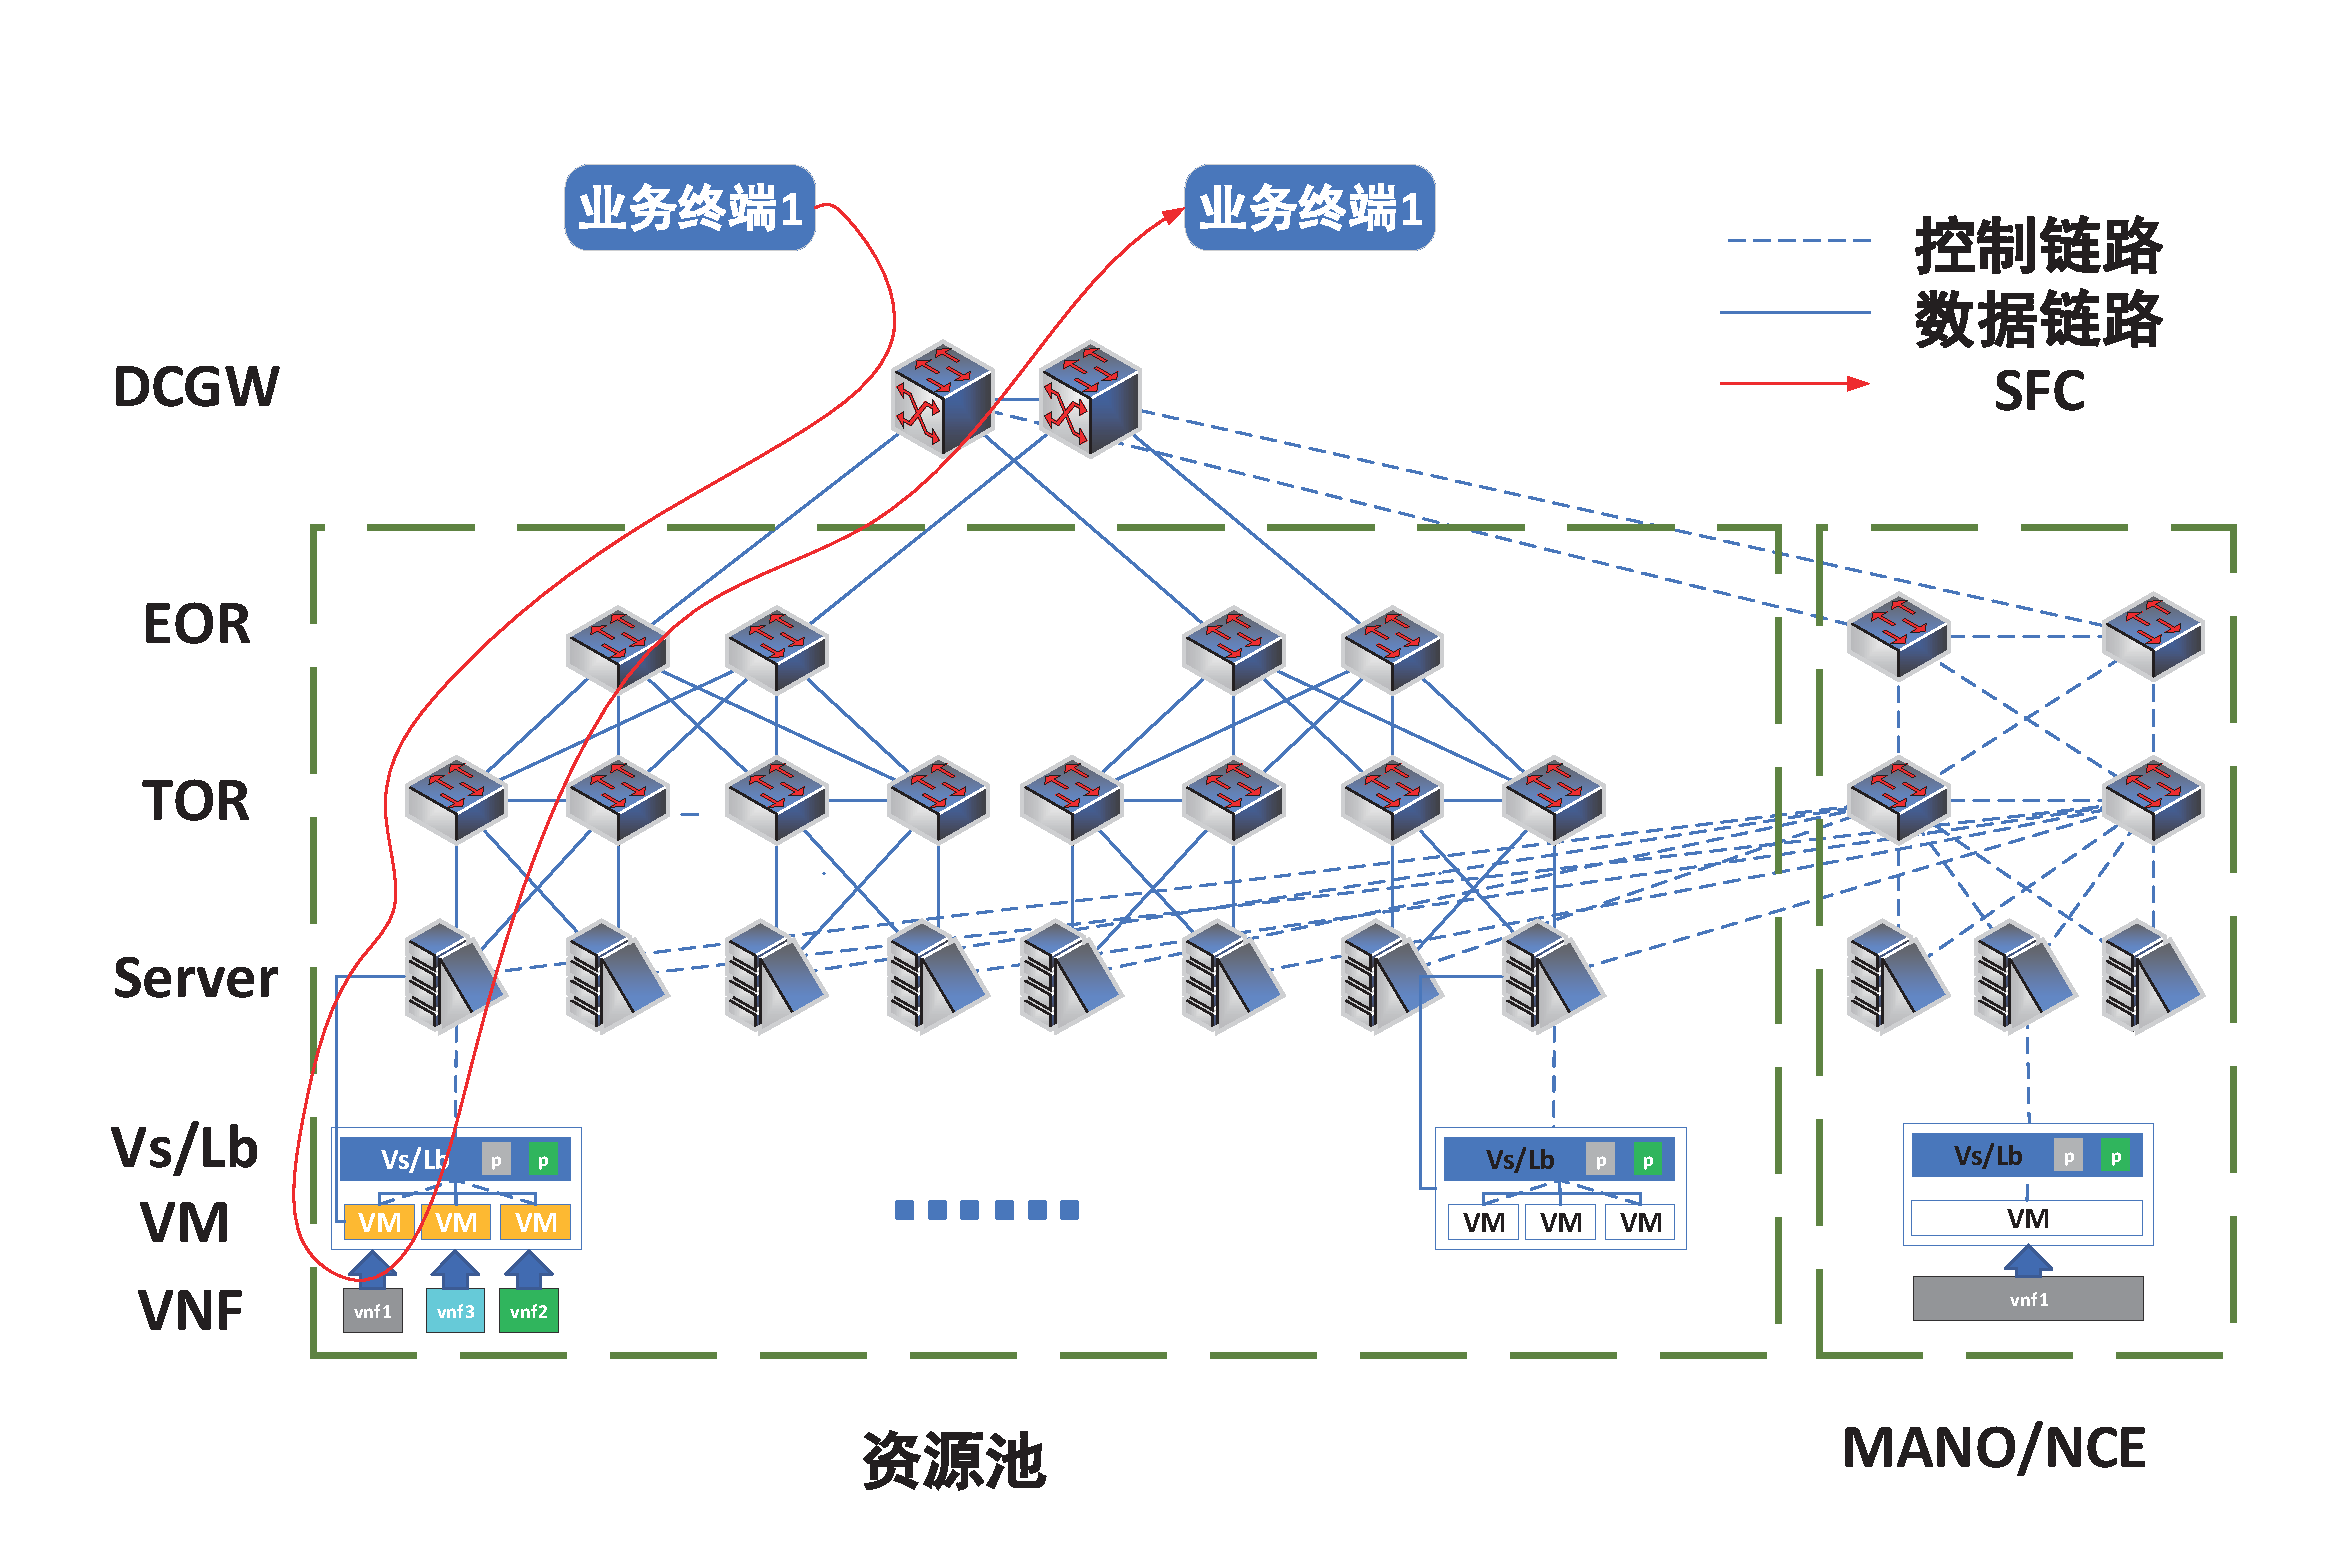
\includegraphics[width = 3in]{img/1.eps}
            \caption{Schematic diagram of cloud virtualization network structure}
            \label{fig1}
        \end{center}
    \end{figure}

    The network evolution model of the cloud-based virtualized network is shown in Fig. \ref{fig2}. At the initial moment, all components in the network are normal. At time $t_1$, a VM node fails, and the VNF carried on the VM node has a backup node. At this time, the service path will be transferred to the standby node, and the original node will wait for repair until the repair is completed at $t_2$.

    \begin{figure}[!t]
        \begin{center}
            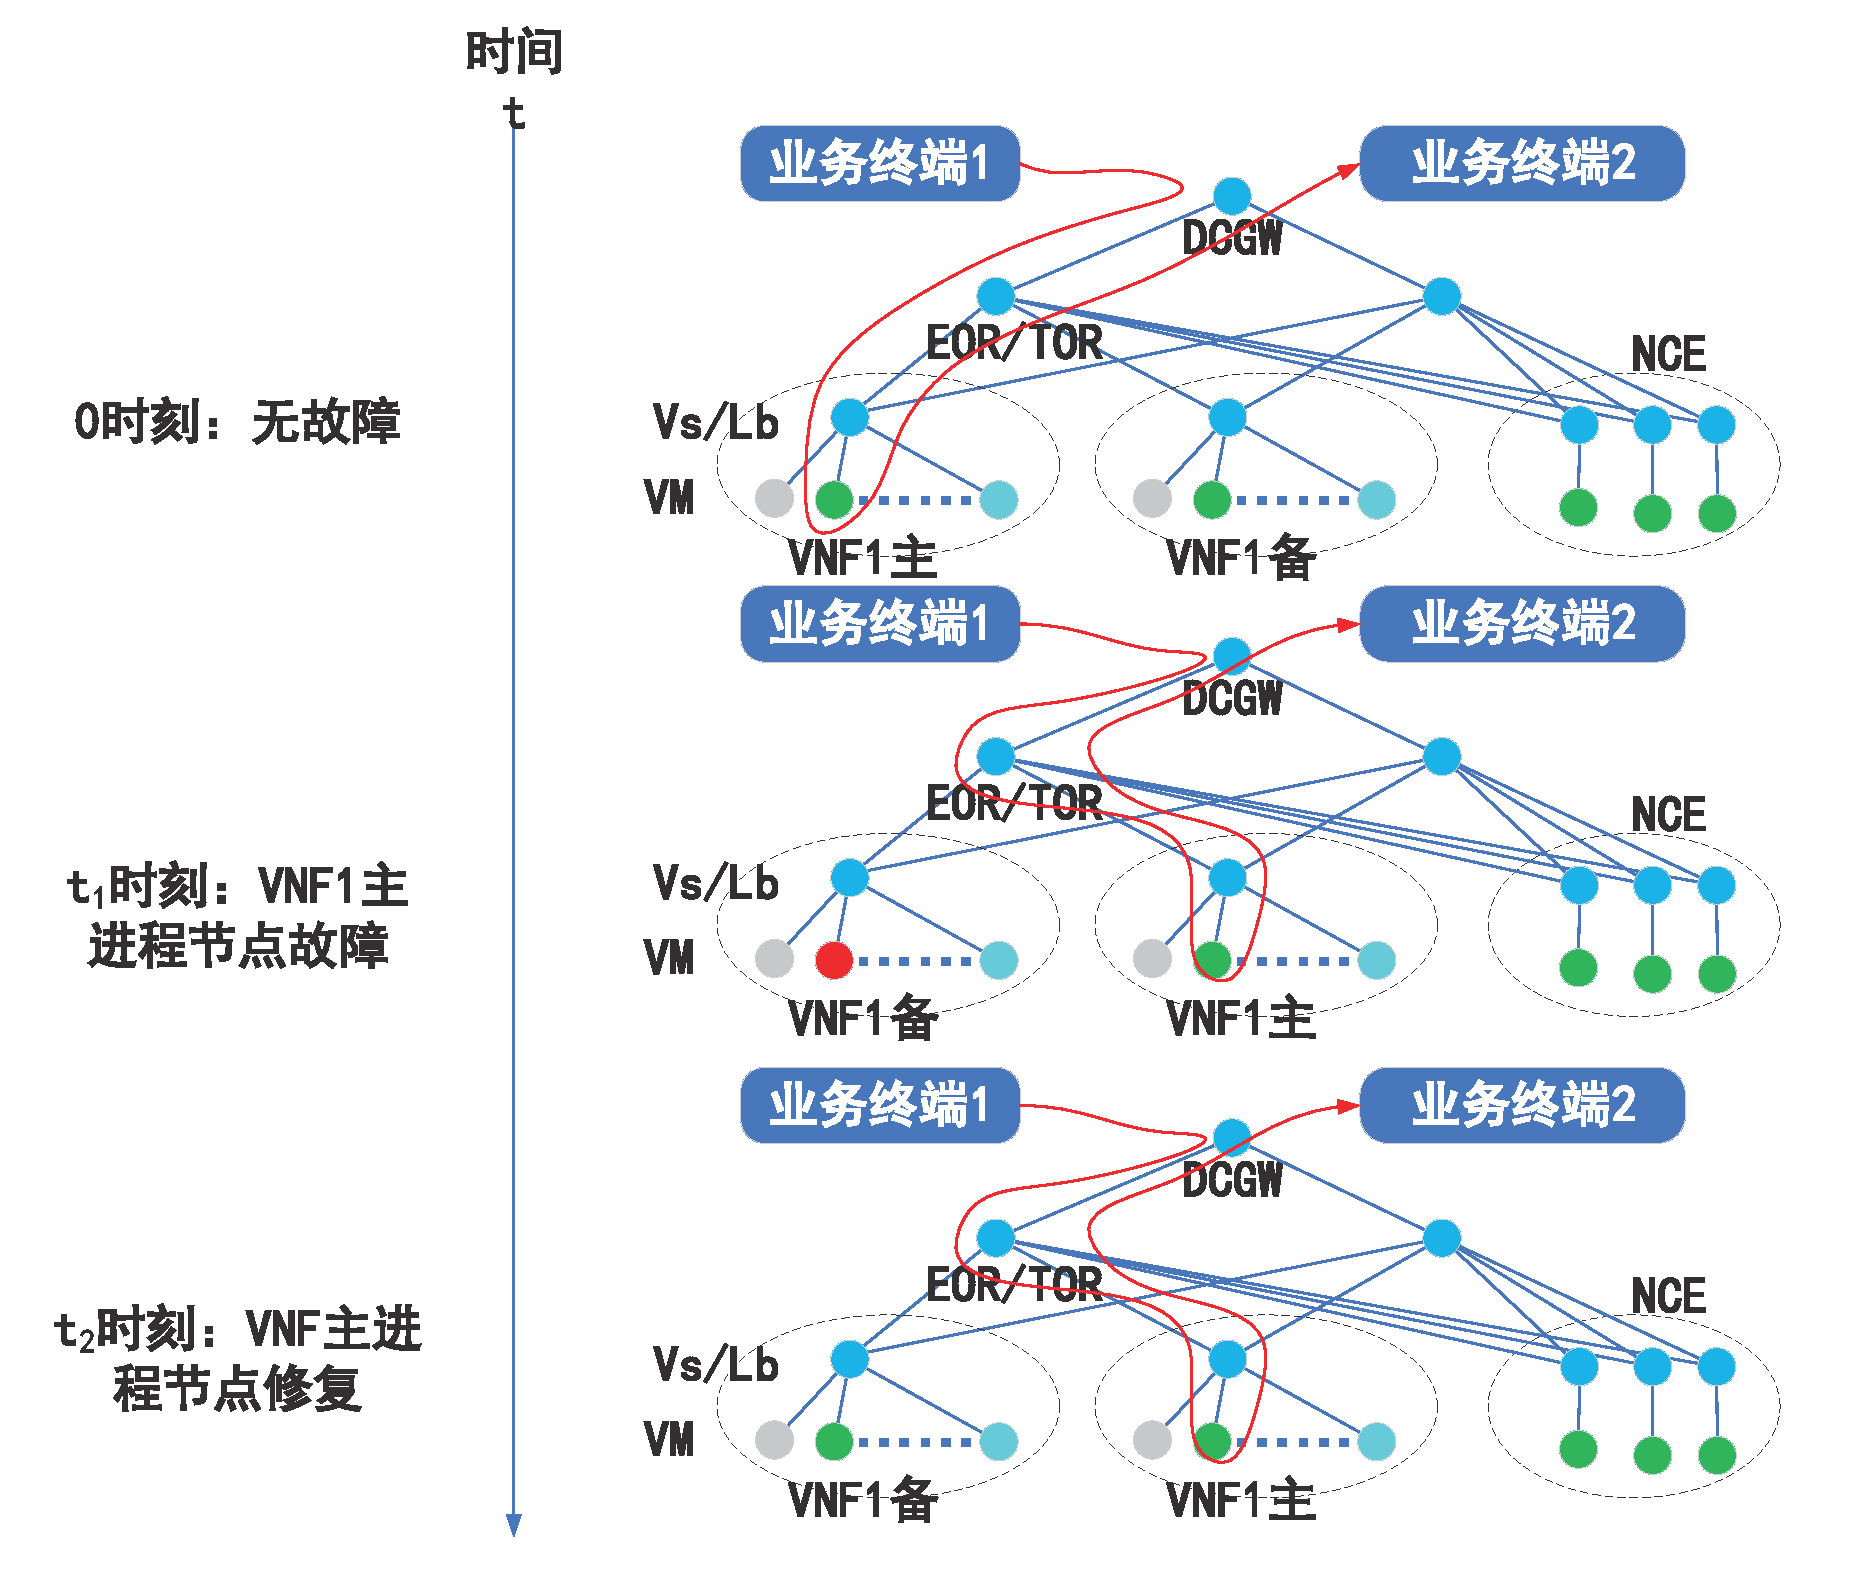
\includegraphics[width = 3in]{img/2.eps}
            \caption{Network evolution model of cloud-based virtualized network}
            \label{fig2}
        \end{center}
    \end{figure}
	
	The network evolution model needs to describe the object of the network evolution. This object not only needs to describe the infrastructure resources of the network physical layer, but also the basic attributes of the network service.
	
    \subsection{Modeling of Cloud and Virtualized Network Evolutionary Objects}

    \subsubsection{Infrastructure layer modeling}
    For cloud-based virtualized networks, the infrastructure layer modeling mainly includes three aspects, namely, network node information, network link information, and network failure mode information.


    Network node information refers to the basic components of the network composed of hardware devices such as Server, VMM, VM, and processes or virtualized software units in the network. In a cloud-based virtualized network, the node types of each network node are heterogeneous, so different network node types need to be described. Here, we divide the network node types into 4 categories: Server nodes, VMM nodes, VM nodes, and Proc nodes (specifically, Proc1, Proc2, and Proc3 nodes correspond to the three different types of services loaded on them). At the same time, the state of the node is used to characterize whether the current state of the node is faulty. Examples of node information are shown in \ref{tab1}, and the red part is an example of table content. For cloud-based virtualized networks, we found through research on relevant information provided by Huawei that network failures mainly occurred on network nodes. At the same time, a network node may have multiple independent failure modes, which will affect the design of subsequent network evolution conditions.

    \begin{table}[!t]
        \renewcommand{\arraystretch}{1.3}
        \caption{Cloud virtualization network node information}
        \label{tab1}
        \centering
        \begin{tabular}{|l||l|}
            \hline
            Symbol       & Discription                                         \\
            \hline
            NodeID       & Describe the unique identifier of the node          \\
            NodeType     & Describe the type of node                           \\
            NodeFailType & The failure mode type of the node                   \\
            NodeFailMTBF & Mean time to failure of the failure type (h)        \\
            NodeFailFDR  & Detection rate after failure                        \\
            NodeFailFDT  & Fault detection time (h)                            \\
            NodeFailAFRR & Probability of automatic repair for software faults \\
            NodeFailAFRT & Automatic repair time for software faults (h)       \\
            NodeFailMTTR & Mean time to repair                                 \\
            NodeFailSR   & Switch Probability                                  \\
            NodeFailST   & Switch Time                                         \\
            NodeState    & Indicates whether the node has failed.              \\
            NodeIdle     & Indicates whether the node is idle                  \\
            Tasp         & Time of calling for check(h)                        \\
            Tchk         & Check time(h)                                       \\
            \hline
        \end{tabular}
    \end{table}

    Network link information refers to the flow path between different nodes in the network. There are two links here, one is the north-south link for sending data from the upper node to the lower node, and the other is the east-west link for mutual control of time and data transfer between nodes of the same kind (for example, for Nway services). That is, the VM node of its business deployment needs to exchange information with the VM node of the flow balancer). For each link, the information of its source and sink nodes is required. At the same time, information about its link capacity and flow is needed. The data dictionary of the link information is shown in \ref{tab2}.

    \begin{table}[!t]
        \renewcommand{\arraystretch}{1.3}
        \caption{Cloud virtualization network link information}
        \label{tab2}
        \centering
        \begin{tabular}{|l||l|}
            \hline
            Symbol              & Discription                     \\
            \hline
            EdgeID              & Describe link unique identifier \\
            EdgeSourceNode      & The source node of the link     \\
            EdgeDestinationNode & The sink node of the link       \\
            EdgeCapacity        & Link capacity (GBp/s)           \\
            EdgeTraffice        & Link flow (GBp/s)               \\
            \hline
        \end{tabular}
    \end{table}

    \subsubsection{Network Application layer modeling}
    In a cloud-based virtualized network, different network elements (Network Function, NF) are combined to form a network service (Netwrok Service, NS), and the network service is a service chain formed by a network service used by two end users  (Service Function Chain, SFC). In order to solve the availability of the service, it is necessary to model the network services invoked by the service and the basic network elements occupied by each network service. The business information of the NFV network can be represented by \ref{tab3}.
    \begin{table}[!t]
        \renewcommand{\arraystretch}{1.3}
        \caption{Cloud virtualization network application information}
        \label{tab3}
        \centering
        \begin{tabular}{|l||l|}
            \hline
            Symbol                 & Discription                                     \\
            \hline
            ApplicationID          & Unique identifier describing the business       \\
            ApplicaitonVNFs        & Describe the SFC called by the application      \\
            ApplicationWorkPath    & Describe the current application link           \\
            ApplicationAvail       & The availability of the application             \\
            ApplicationDownTime    & Cumulative unavailable time of business         \\
            ApplicationStatus      & Describe whether the current business is normal \\
            ApplicationInitTraffic & Record initial traffic                          \\
            ApplicationTraffic     & Describe the relative value of current traffic  \\
            ApplicationThreshold   & Describe the minimum flow threshold             \\
            \hline
        \end{tabular}
    \end{table}

    Services will call different VNFs. These VNFs are divided into three different types according to their backup conditions: non-backup services, cold backup services, and hot backup services. They are deployed on different types of VM nodes. For network services, since this project mainly focuses on whether the service is interrupted, the service attributes can be designed as shown in \ref{tab4}.
    \begin{table}[!t]
        \renewcommand{\arraystretch}{1.3}
        \caption{Cloud virtualization network VNF information}
        \label{tab3}
        \centering
        \begin{tabular}{|l||l|}
            \hline
            Symbol        & Discription                              \\
            \hline
            VNFID         & The unique identifier of the network VNF \\
            VNFBackupType & Service backup types                     \\
            VNFDeployNode & Master nodes of the VNF                  \\
            VNFBackupNode & Slayer nodes of the VNF                  \\
            VNFFailSR     & Switch rate                              \\
            VNFFailST     & Switch time                              \\
            VNFSwitchPath & Switch Path                              \\
            VNFWait       & The state of the VNF                     \\
            \hline
        \end{tabular}
    \end{table}

    \subsection{The evolution conditions of cloud virtualised network}
    Network evolution conditions are mainly caused by the interruption of top-level network services under different failure modes of different devices. At the same time, the network failure of the top node will cause the failure of the bottom node according to a certain probability. At the same time, network nodes will be repaired due to automatic repair and manual repair. Therefore, the main ideas for the design of network evolution conditions are as follows:

    1. For each network node, it is assumed that the time probability distribution of failure, automatic repair, and manual repair are all exponentially distributed. First, according to the different failure modes occurring on it, the node state sequence corresponding to the failure mode is generated respectively. For example, for the H1 node, there are two failure modes. According to the MTBF of failure mode 1, the duration before a failure is generated. Then determine whether the fault is detected. If it is not detected, the fault will exist until the inspection time (168 hours); if it is detected, it will be judged whether it is automatically repaired or manually repaired according to the probability of automatic repair, and the repair time will be given. . Finally, the failure state sequence of failure mode 1 is synthesized.

    2. For all failure modes of each node's failure, the failure state sequence of the node is given, that is, the failure state sequence of all failure modes is combined.

    3. Give the node that fails at each moment.

    \begin{figure}[!t]
        \begin{center}
            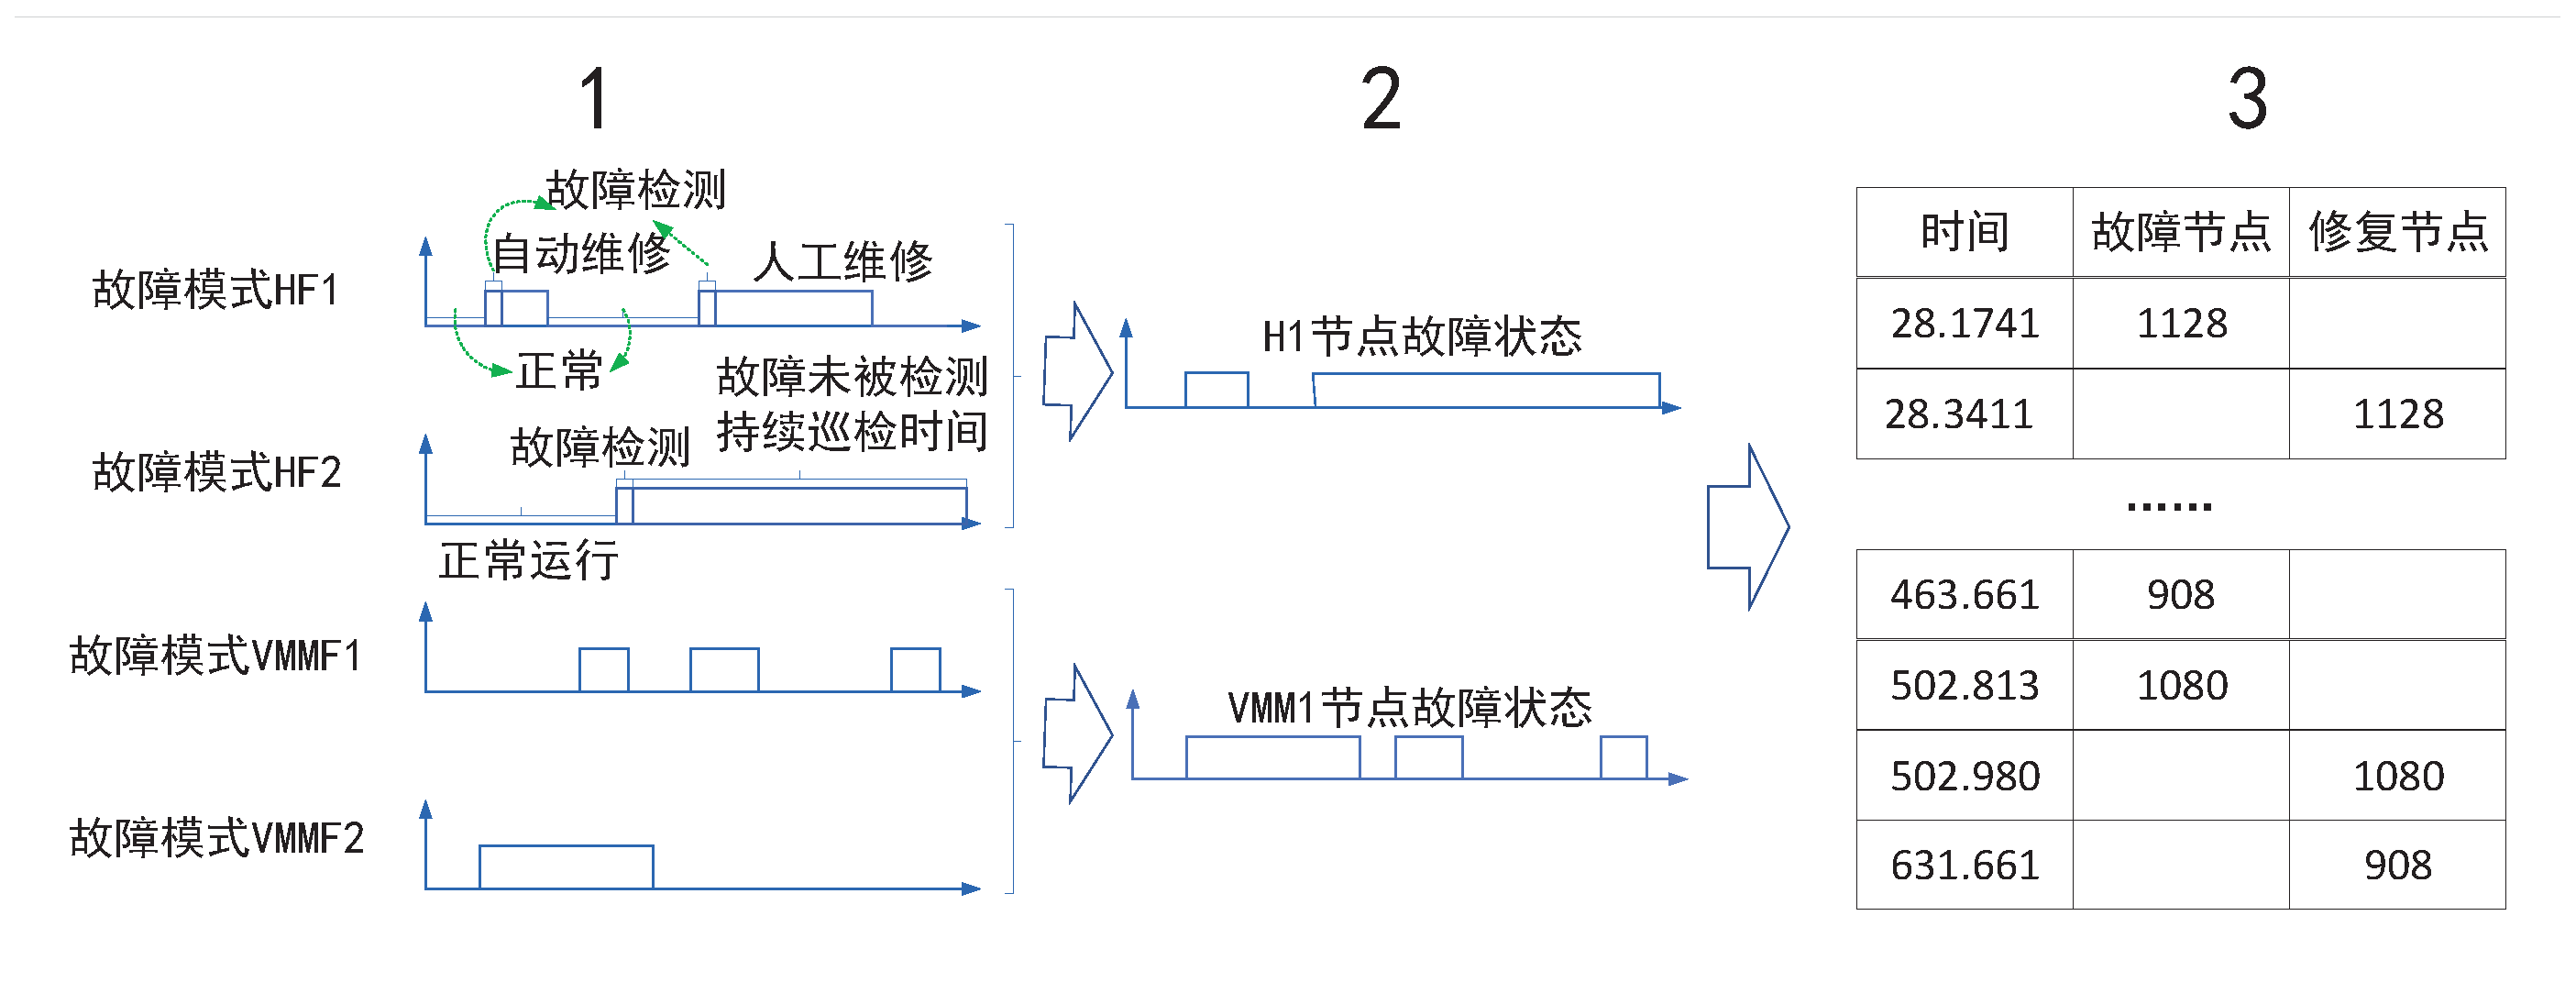
\includegraphics[width = 3in]{img/3.eps}
            \caption{The evolution conditions of cloud virtualised network}
            \label{fig3}
        \end{center}
    \end{figure}

    \subsection{The evolution rules of cloud virtualised network}

    \subsubsection{DCGW/EOR/TOR}
    When a switch node fails, the service traffic of different services carried by it is interrupted, and the service carried by it experiences a failure with a duration of NodeFailST.

    \subsubsection{Server}
    When a Server node fails, all its downstream software nodes fail. At this time, the migration of all VMs and proc nodes hosted on it will be triggered. At this time, if the migration is successful, all nodes and services on it experience a failure of NodeFailST time, and the Server node enters the maintenance state, and becomes an idle Server node after repair. If the migration fails, or there is no idle server, all nodes on it experience a failure time of NodeFailMTTR.

    \subsubsection{Vs/Lb}
    When a Vs/Lb node fails, the traffic of all VM nodes and services in the server is interrupted. Since Vs/Lb contains forwarding and control functions, all VM nodes and business traffic cannot occur

    \subsubsection{VM}
    When a VM node fails, different maintenance and protection strategies will be determined according to the type of the node and its subordinate VNF.

    For a VNF without backup, it waits for the original fault to be repaired after it fails, and there is no additional rule. At this time, the failure time is the duration of the failure.

    For a cold backup VNF, when the main VM node fails, it is judged whether the switchover can be successful. If the backup VM node does not fail and the switchover is successful, the failure time is the switchover time, and the primary node becomes the standby node after the failure is repaired; if the switchover fails or the standby node fails, wait for the failure of the primary node to disappear, and the failure time is the time of the primary node. Fault repair time.

    \begin{figure}[!t]
        \begin{center}
            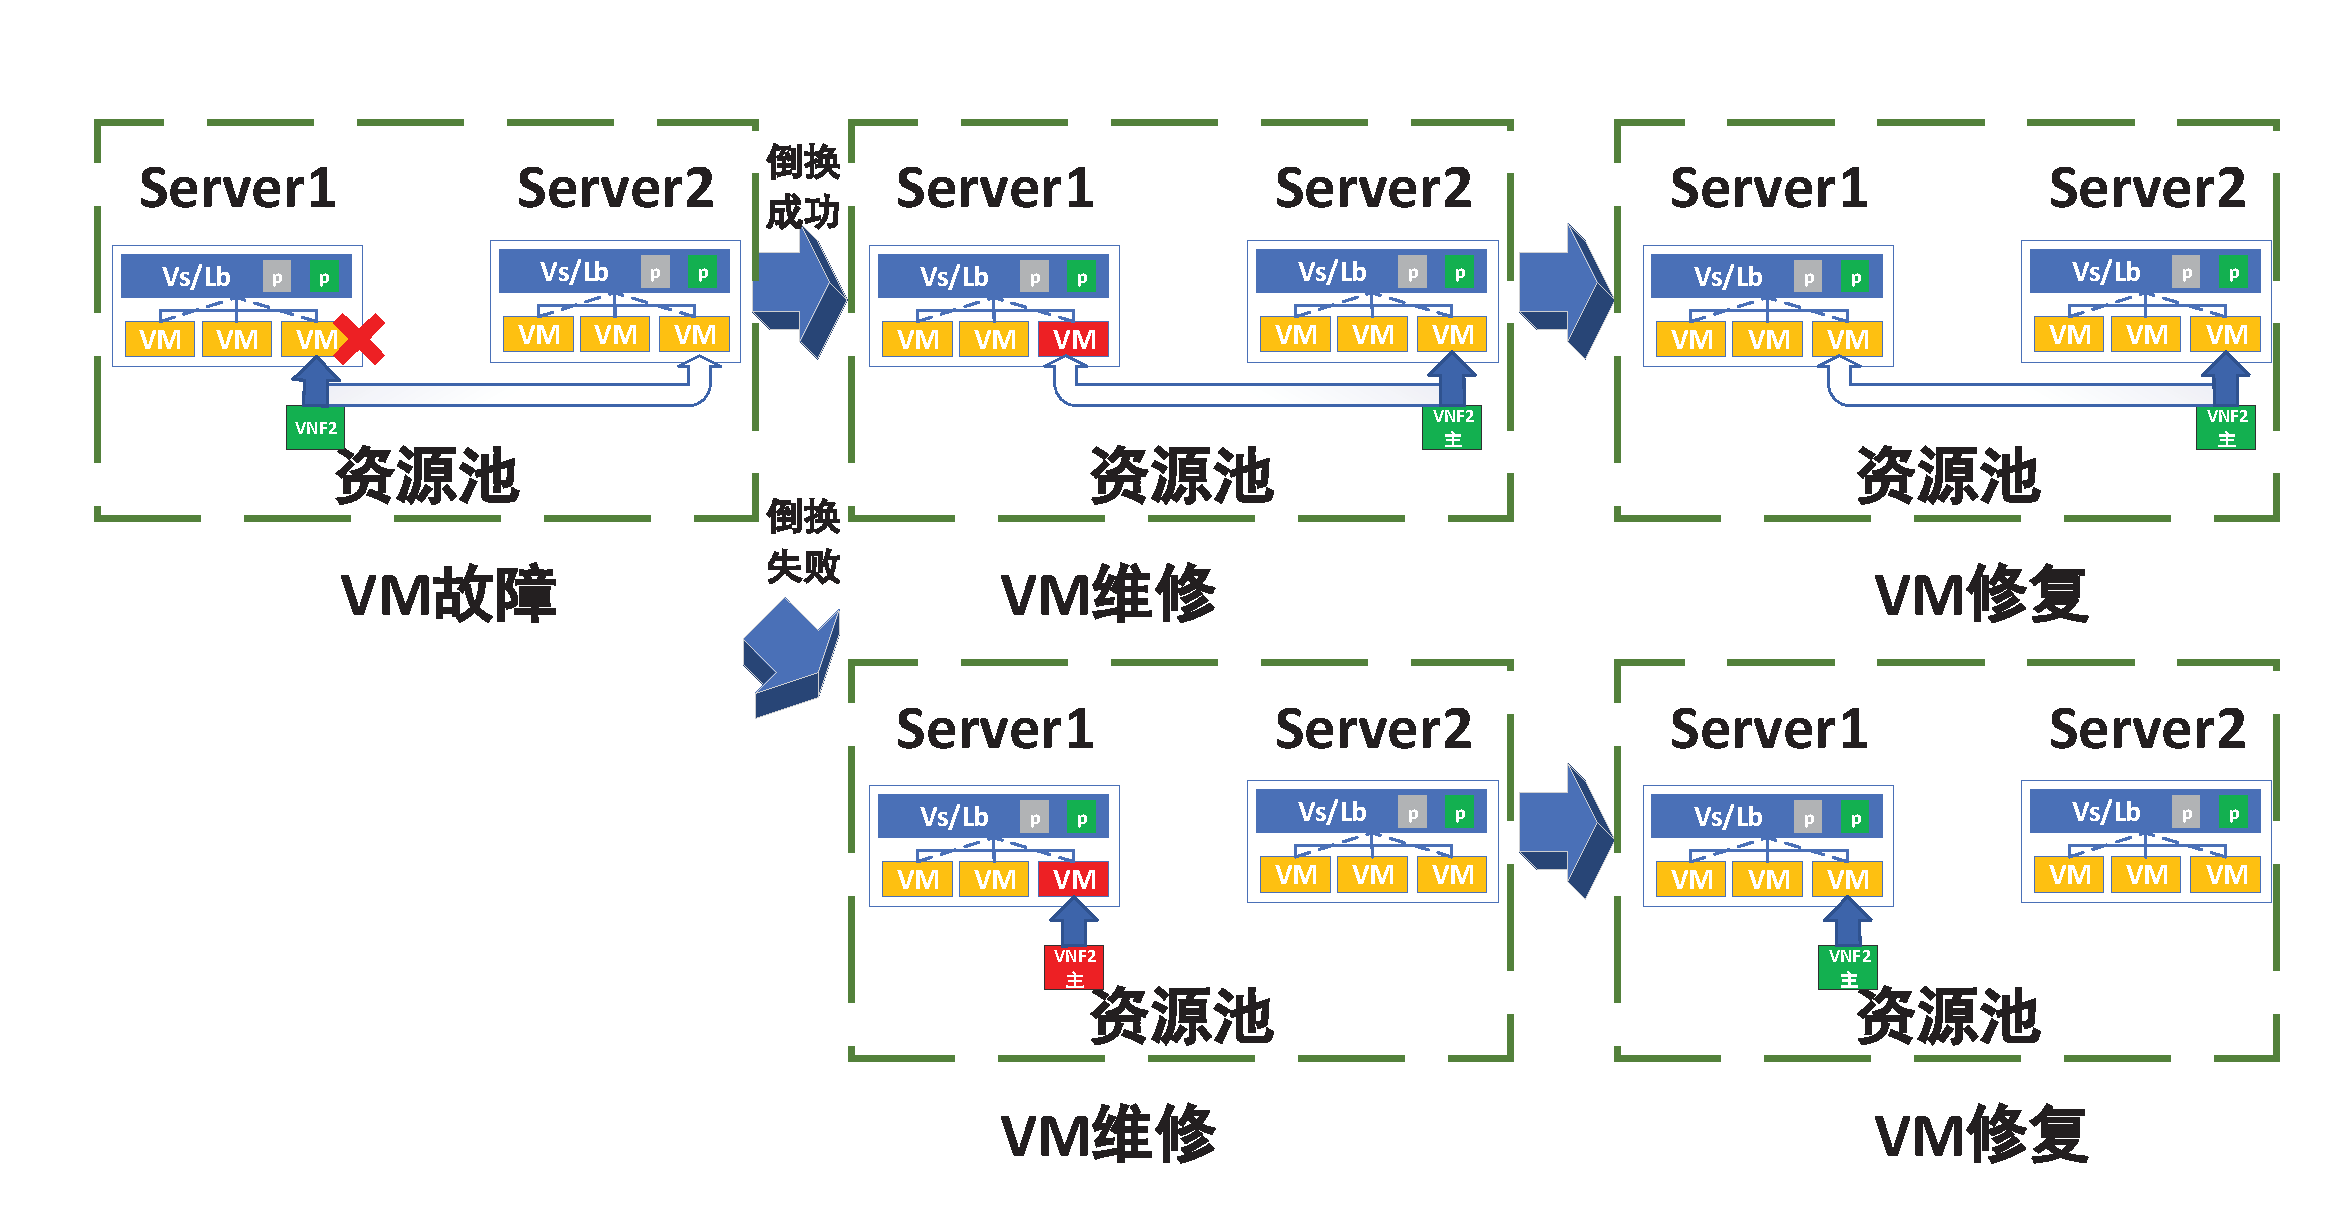
\includegraphics[width = 3in]{img/7.eps}
            \caption{The cold backup VNF process fails}
            \label{fig4}
        \end{center}
    \end{figure}

    For a hot backup VNF, when any of its working VM nodes fails, it is judged whether the switchover is successful. If the switch is successful, the traffic of the node is switched to the other two nodes, and the switch is performed when the node fails. At this time, the VNF fails with 2 NodeFailST; and when the switch fails, the VNF fails, and the business failure time It is the failure recovery time of the node.

    \begin{figure}[!t]
        \begin{center}
            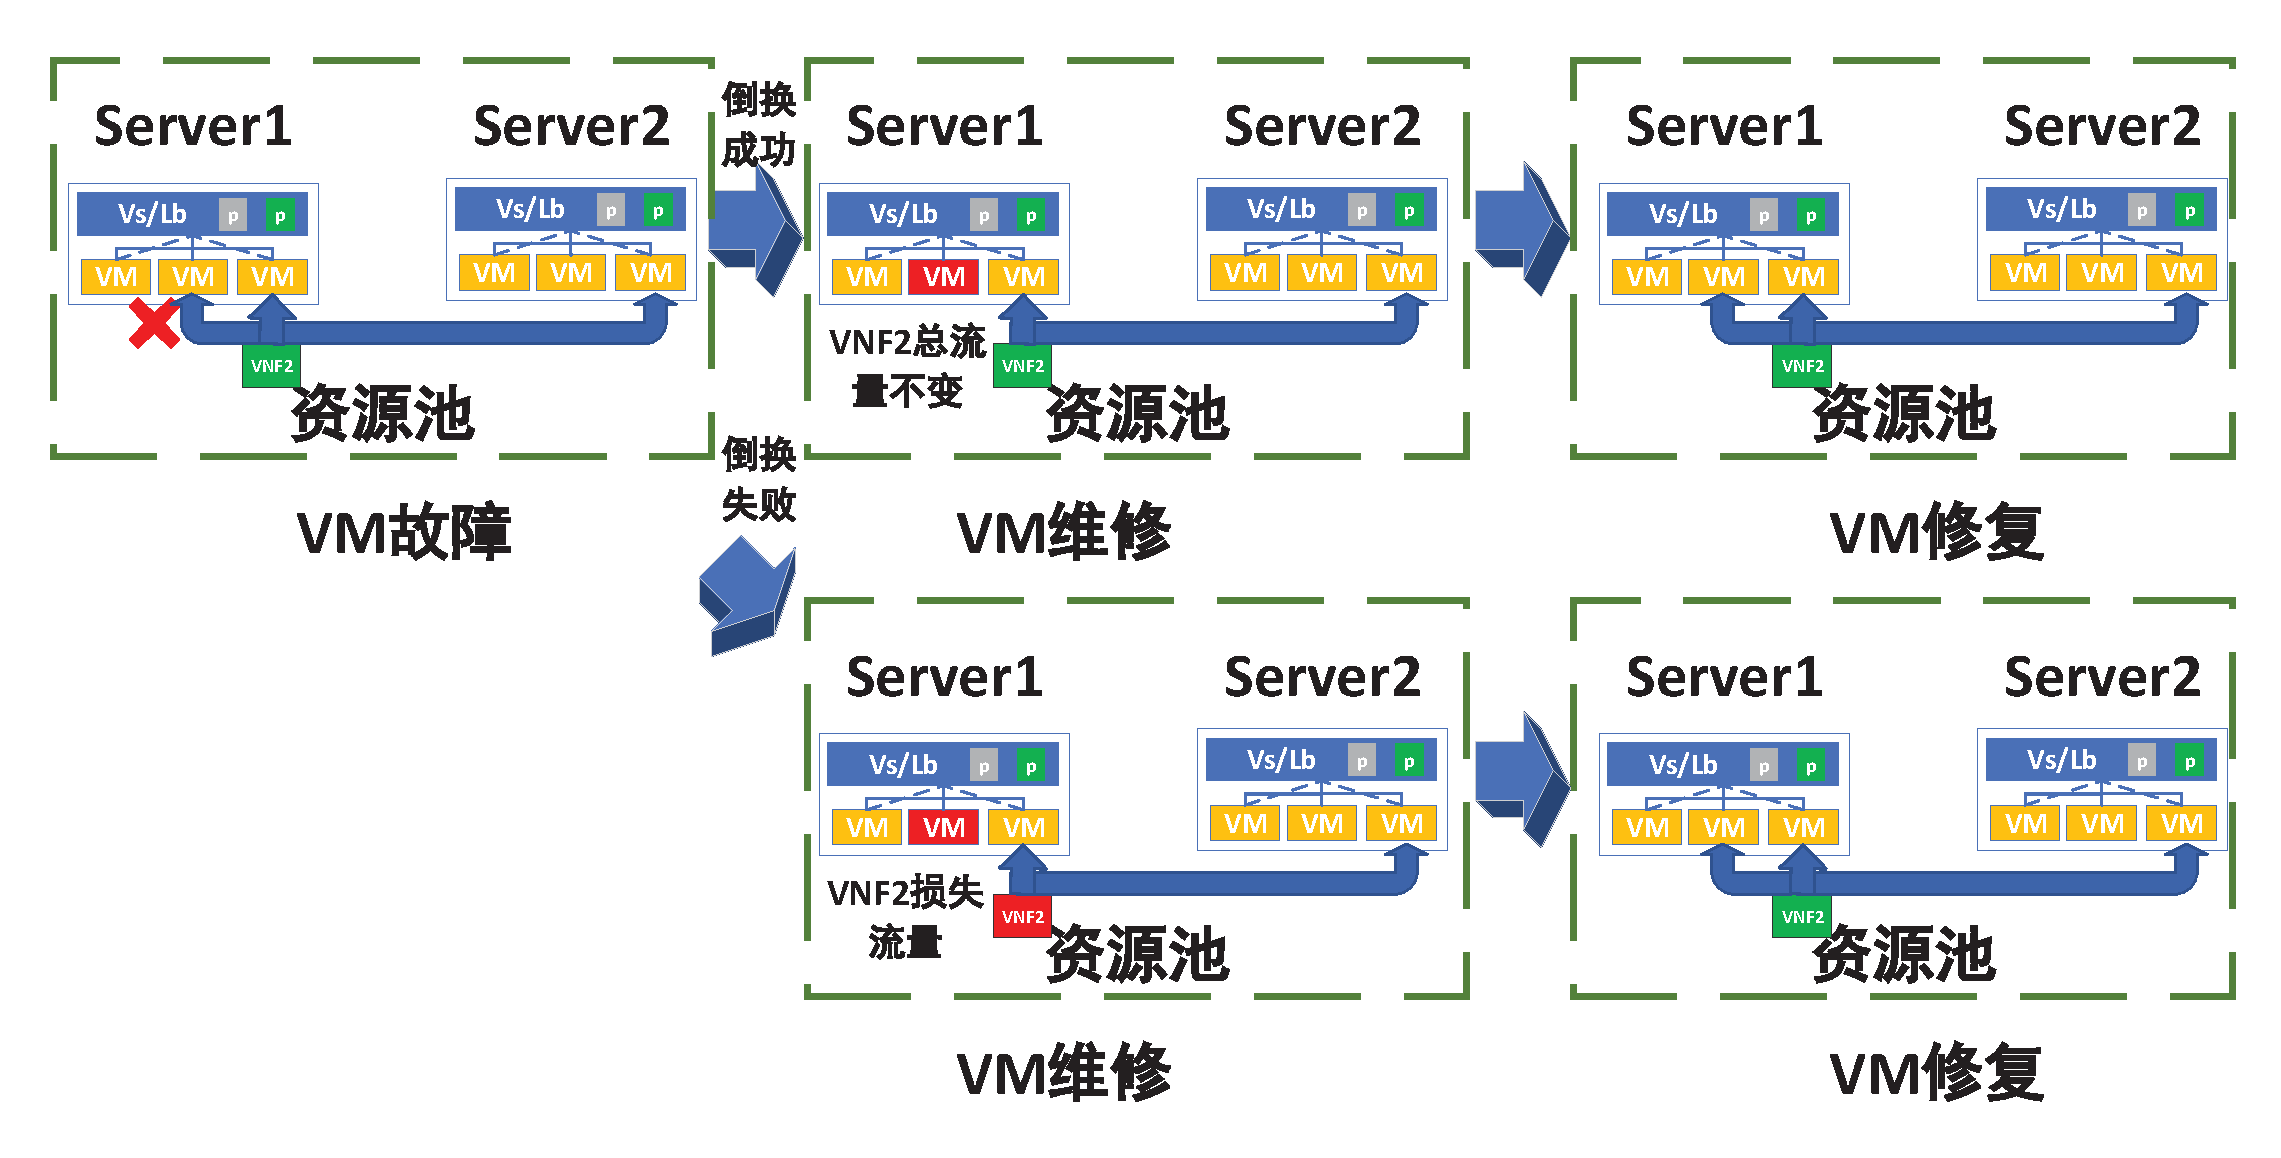
\includegraphics[width = 3in]{img/8.eps}
            \caption{The hot backup VNF process fails}
            \label{fig5}
        \end{center}
    \end{figure}


    \section{Reliability Evaluation of Cloud Virtualization Network}
    The algorithm flow of cloud virtualization network reliability evaluation is shown in Figure \ref{fig6}.


    The overall reliability calculation module of the network starts with the input of the cloudized virtual network, business information, calculation times and calculation cycle data from the very beginning. At this time, the software begins to model the evolution object and initialize it, and automatically generate the evolution state of the fault data according to the network information, generate the set of faulty nodes at each time, and the set of restored nodes at each time.

    The loop starts at this time, and each loop is a Monte Carlo simulation.

    First traverse the set of recovery nodes. For the business involved in each node, if the cumulative failure time of the business is non-zero, the failure occurrence time is added to the cumulative failure occurrence time of the business.

    After completing the traversal of the restored node, start traversing the failed node, and according to the type of the node, determine the processing rules after the node failure, and jump to the corresponding program, if the type of the failed node is DCGW/EOR/TOR, etc., then jump to Switch node fault handling module.

    After traversing the faulty node, the reliability calculation of all services is started. The reliability of the i-th service is $1-(\sum App\_unavailtime^i(t)/T)$, and the reliability of the entire network is $R_{Application}(T)=\sum_i^{N_{Application}}w_iR_A ^i(T)$ At this time, a simulation cycle is completed, and the cycle counts i+1, and loops until i reaches the expected number of calculations input.

    After completing the simulation of the expected number of calculations, the business reliability of the i-th service is $R_A^i(T)/N$, and the reliability of the entire network is $R_{Application}(T)/N$.

    \begin{figure}[!t]
        \begin{center}
            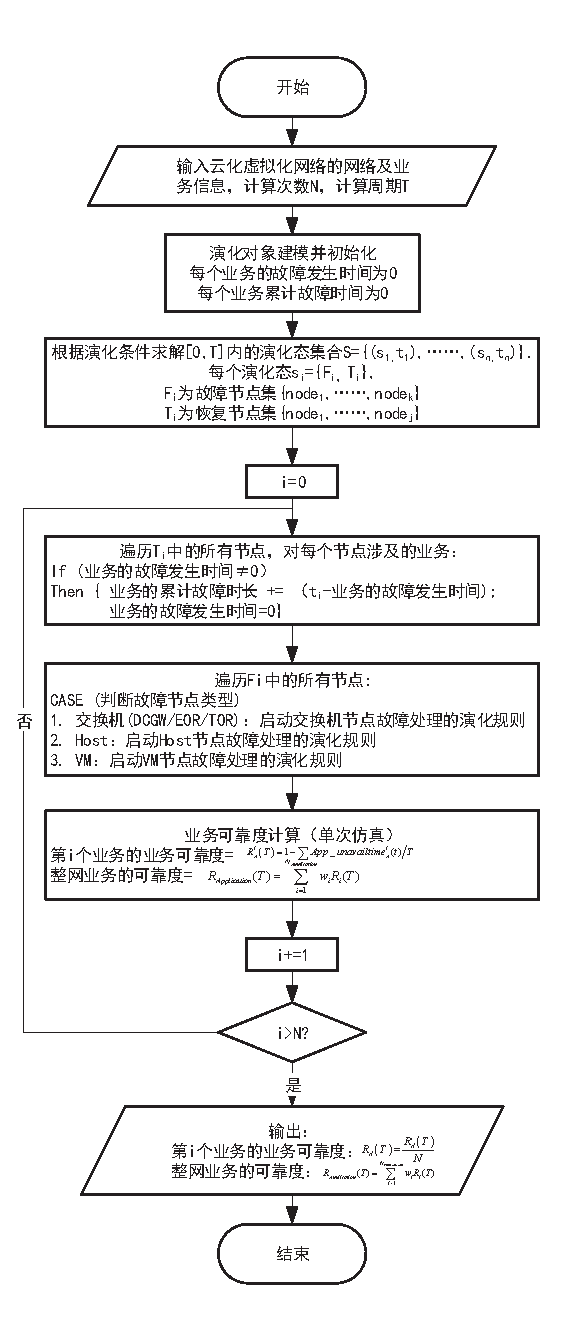
\includegraphics[width = 3in]{img/9.eps}
            \caption{Reliability evaluation model}
            \label{fig9}
        \end{center}
    \end{figure}


    \section{Case analysis and discussion}
    In this part, we first constructed a typical cloud-based virtualized network case, in which a certain number of VNFs and network services were randomly deployed, and then selected typical network services to analyze the stability of the results of the calculation model, and use this article The proposed model calculates the reliability of a single network service and the entire network service.

    \begin{figure}[!t]
        \begin{center}
            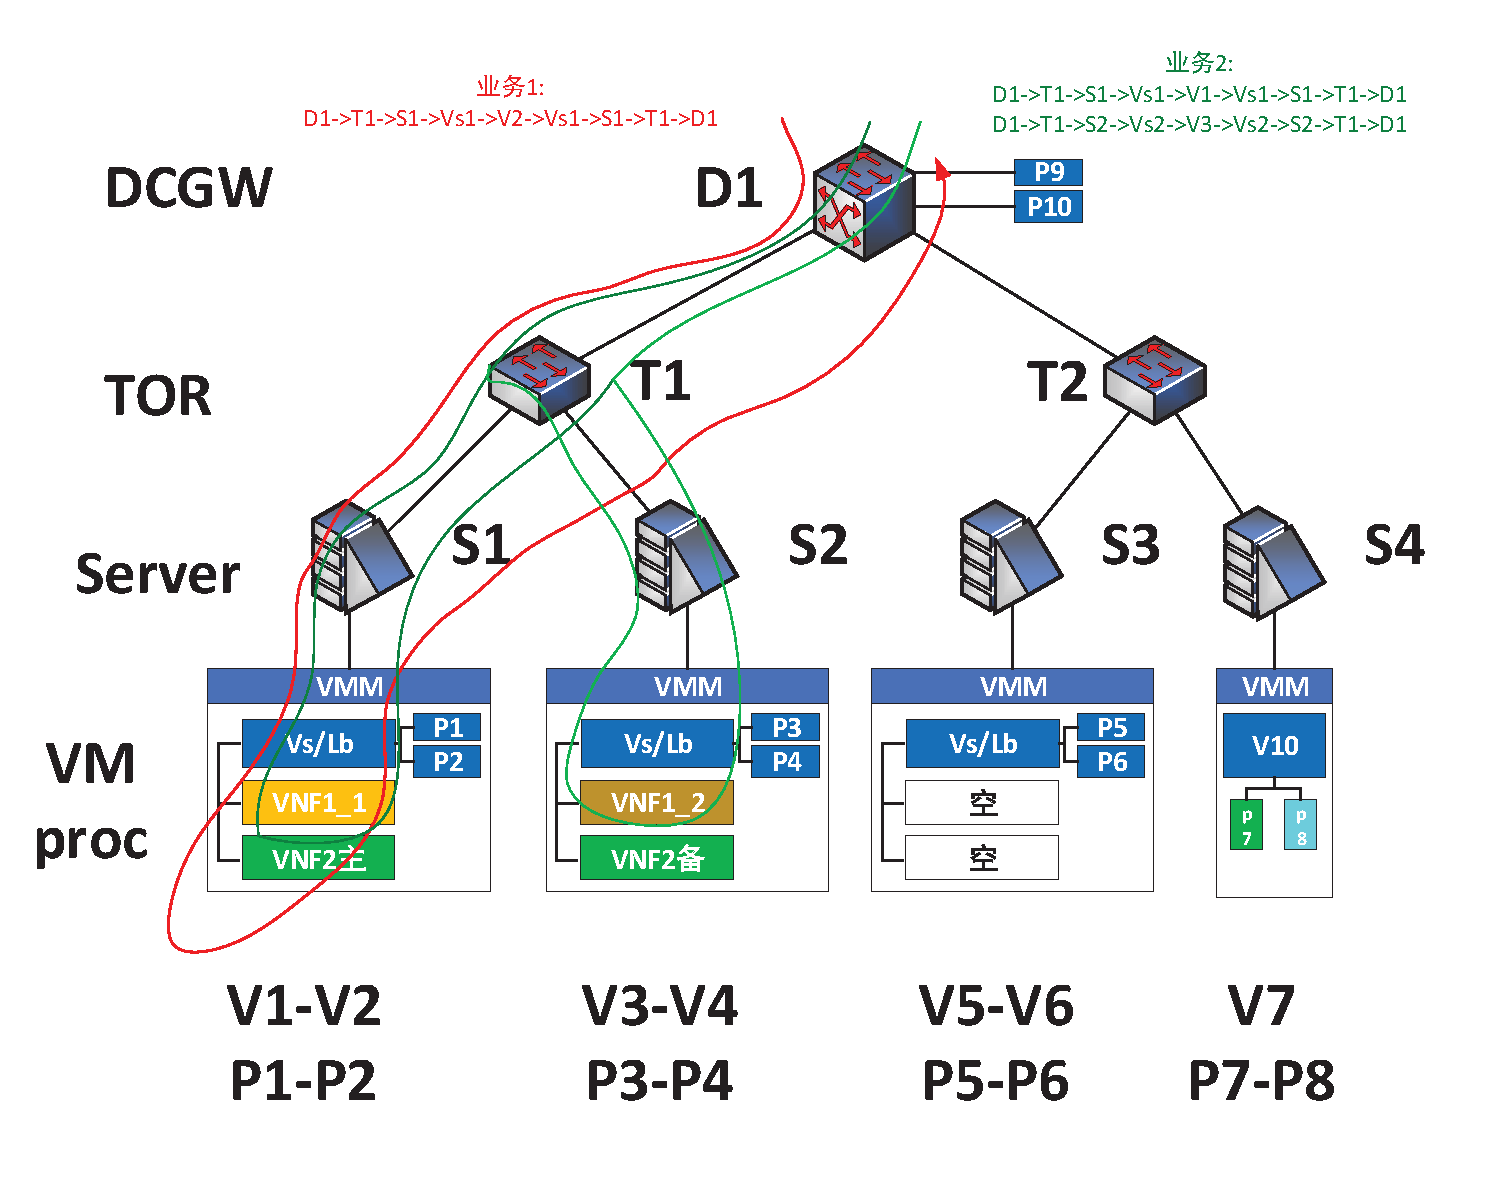
\includegraphics[width = 3in]{img/11.eps}
            \caption{Small network case topology}
            \label{fig10}
        \end{center}
    \end{figure}

    \begin{figure}[!t]
        \begin{center}
            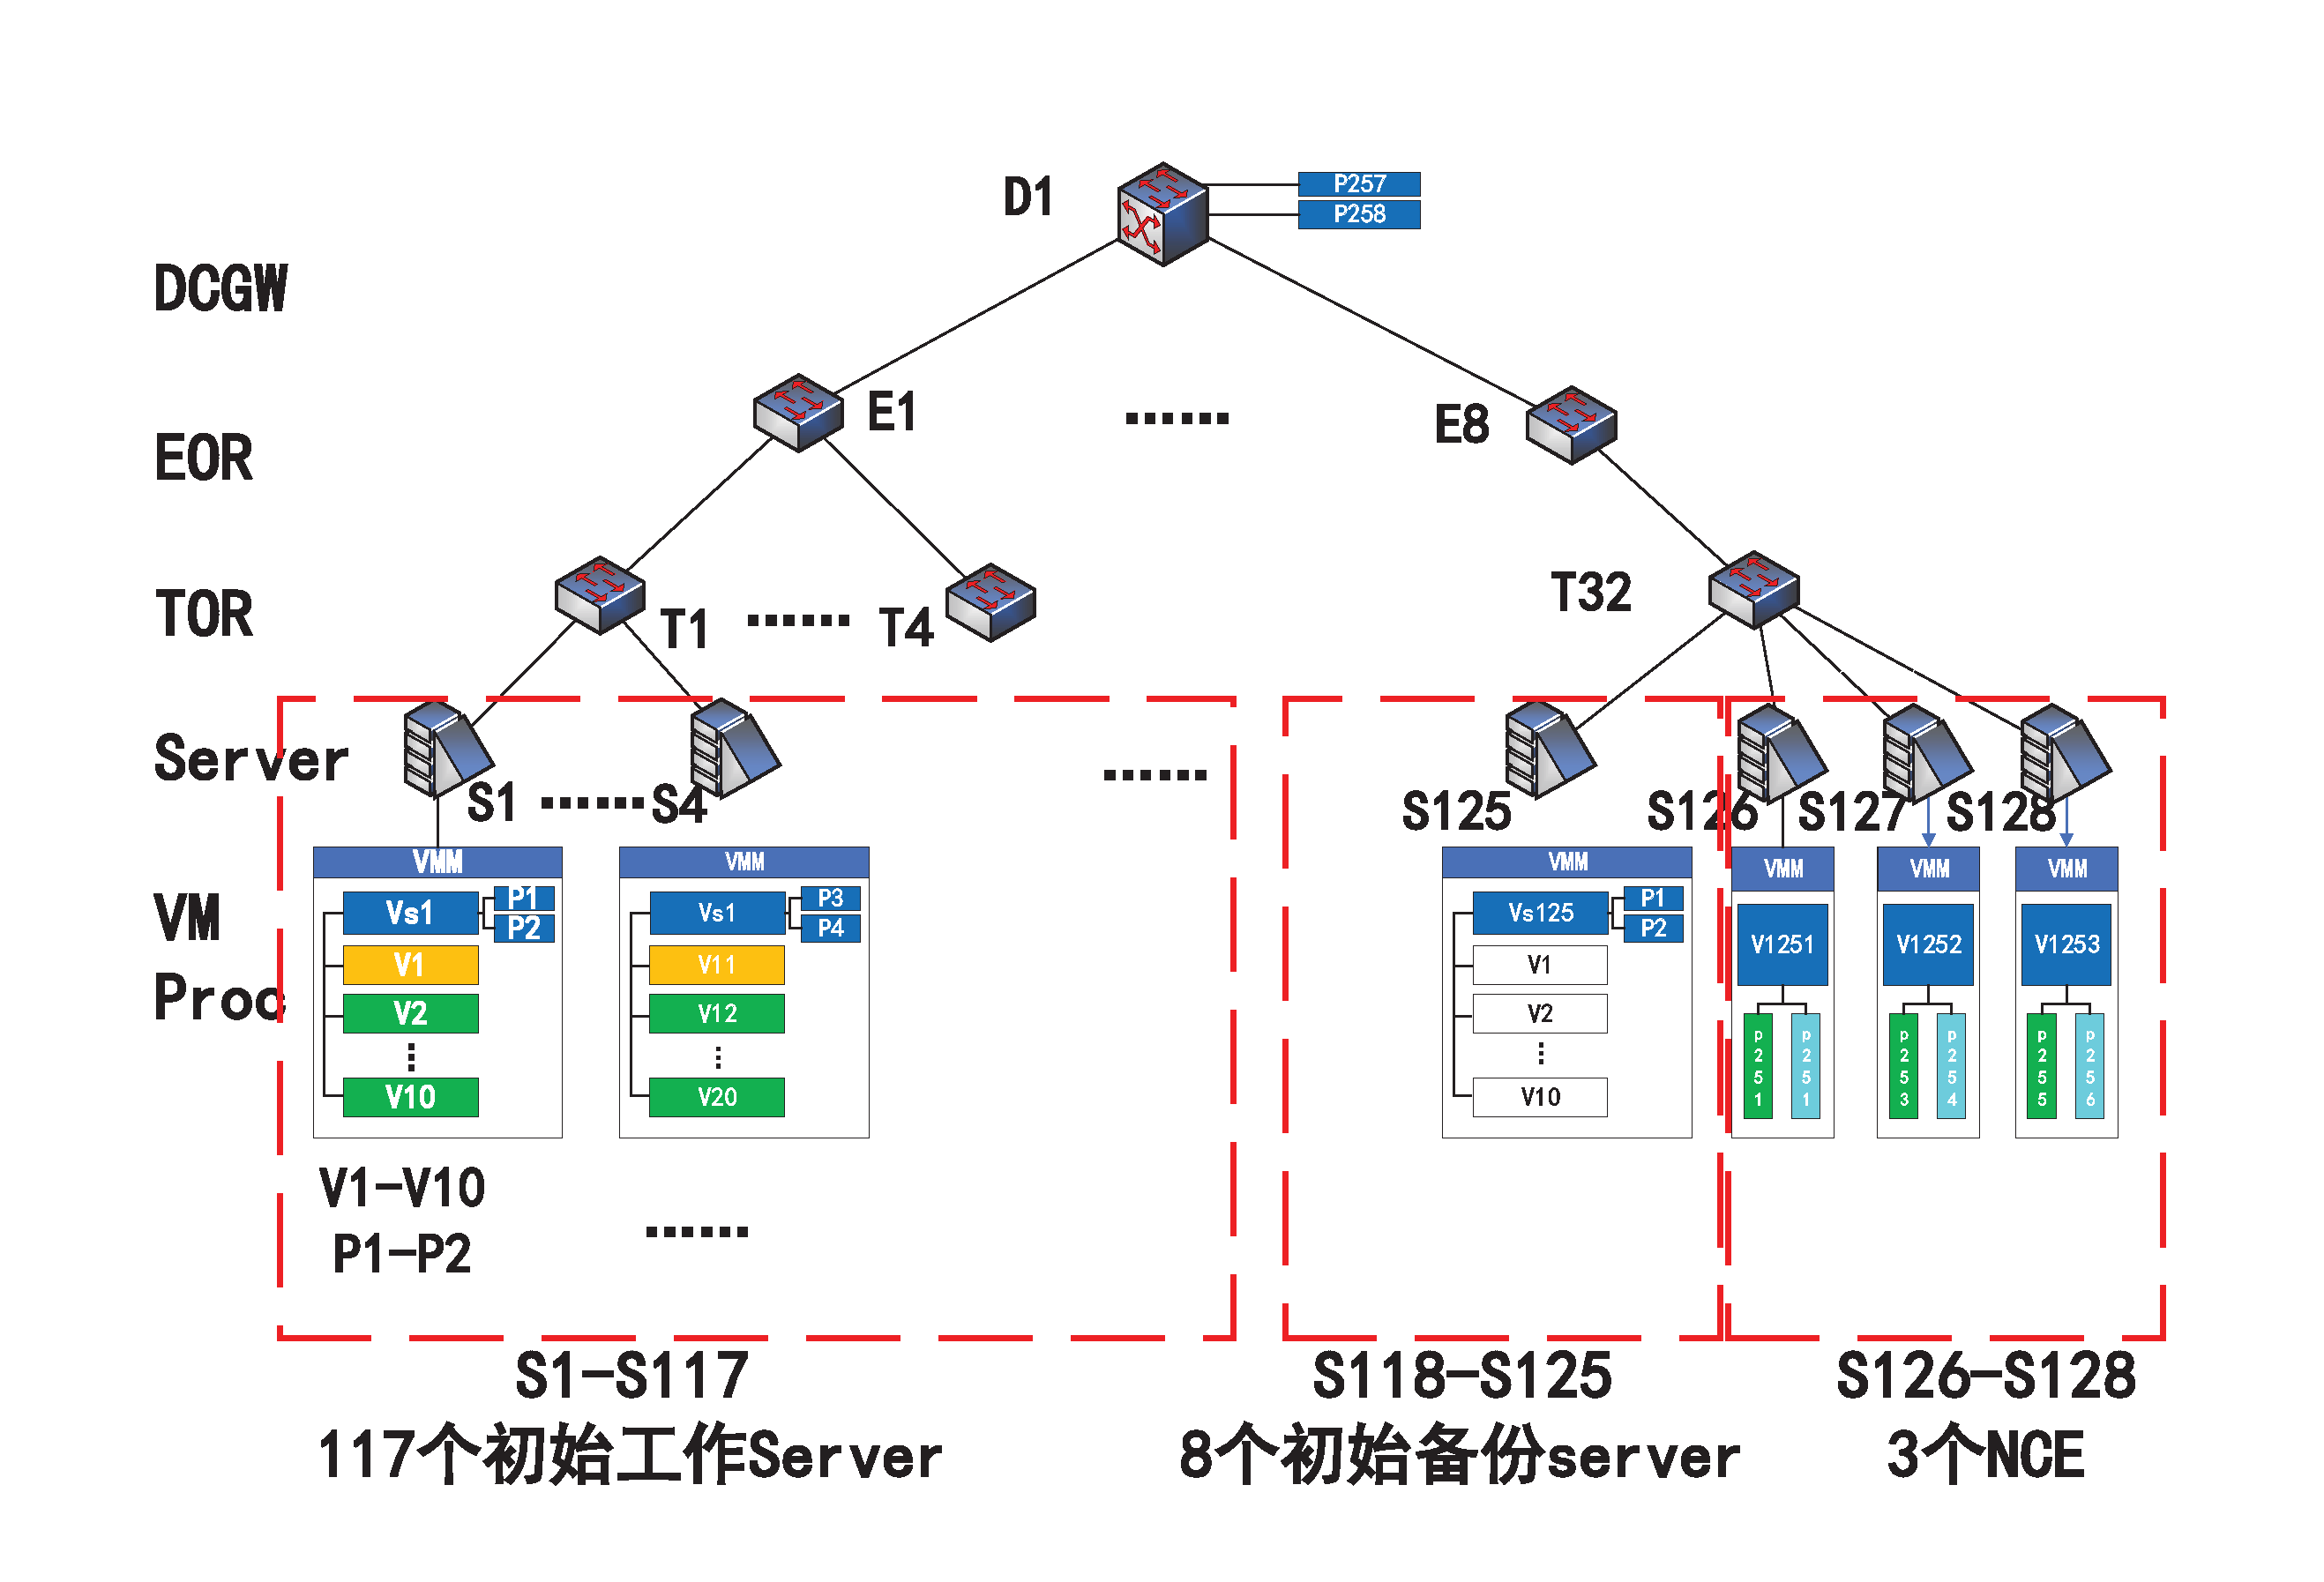
\includegraphics[width = 3in]{img/10.eps}
            \caption{Large network case topology}
            \label{fig11}
        \end{center}
    \end{figure}

    In this case, each node sets its node parameters according to its node type. The relevant parameters of each type of node are shown in Table 5.


    In order to compare the traditional reliability calculation methods, we have designed a small network case (as shown in Figure \ref{fig10}) for calculation. Two types of VNF are deployed in the figure. VNF1 is a 2 Way backup VNF, and VNF2 is a backup VNF of the active backup type. There are two services in the network.

    \begin{table}[!t]
        \renewcommand{\arraystretch}{1.3}
        \caption{Case parameter setting}
        \label{tab5}
        \centering
        \begin{tabular}{|c|c|c|c|c|c|c|}
            \hline
            Type    & MTBF  & FDR & FDT & AFRR & AFRT  & MTTR  \\
            \hline
            DCGW    & 50   & 1   & 0s  &      & 2h    &      \\
            TOR     & 50   & 1   & 0s  &      & 2h    &      \\
            Server  & 50   & 1   & 0s  &      & 2h    &      \\
            Vswitch & 2    & 0.9 & 0s  & 0    & 10min & 2h   \\
            VM      & 2    & 0.9 & 0s  & 0    & 10min & 2h   \\
            Proc    & 20   & 0.9 & 0s  & 0    & 10min & 2h   \\
            \hline
        \end{tabular}
    \end{table}

    As shown in Figure \ref{Figure 11}, we have constructed a cloud virtualization network model consisting of 1 DCGW node, 8 EOR nodes, 32 EOR nodes and 128 Server nodes. Among them, there are 125 service servers, and each server has 10 VMs; 3 servers are used as NCE services.

    \begin{table}[!t]
        \renewcommand{\arraystretch}{1.3}
        \caption{Case parameter setting}
        \label{tab5}
        \centering
        \begin{tabular}{|c|c|c|c|c|c|c|}
            \hline
            Type    & MTBF & FDR & FDT  & AFRR & AFRT & MTTR \\
            \hline
            DCGW    & 50y   & 1 & 15s  &      &   	& 2h     \\
            TOR     & 50y   & 1 & 15s  &      &    &   2h   \\
            Server  & 50y   & 1 & 15s  &      & 	   &  2h    \\
            Vswitch & 2y    & 1 & 240s & 0.9    & 10m   & 2h   \\
            VM      & 2y    & 1 & 240s & 0.9  & 10m   & 2h   \\
%            Proc    & 20y   & 0.9  & 240s  & 0.9  & 10m   & 2h   \\
            \hline
        \end{tabular}
    \end{table}

    In this network, 147 VNFs are randomly deployed on 1170 VMs on S1-S117, which are divided into three categories: 1) 60 mainframe VNFs; 2) 29 active and standby VNFs; 3) 58 2 way type VNF. The specific parameters of VNF are shown in Table 9 in the appendix.


    We randomly select VNFs to combine to form 100 businesses. Among them: 1) 30 services including only 1 VNF; 2) 40 services including 2 VNFs; 3) 30 services including 3 VNFs. The specific parameters of the business are shown in Table 10 in the appendix.

    \subsection{Algorithm correctness analysis}
    In the traditional method, the reliability of the virtual network infrastructure (NFVI) and virtual link (Vlink) deployed by the VNF and VNF is often calculated through the RBD method. According to the ETSI report [7], two business reliability block diagrams in two cases can be given as shown in \ref{Figure 12}.

    \begin{figure}[!t]
        \begin{center}
            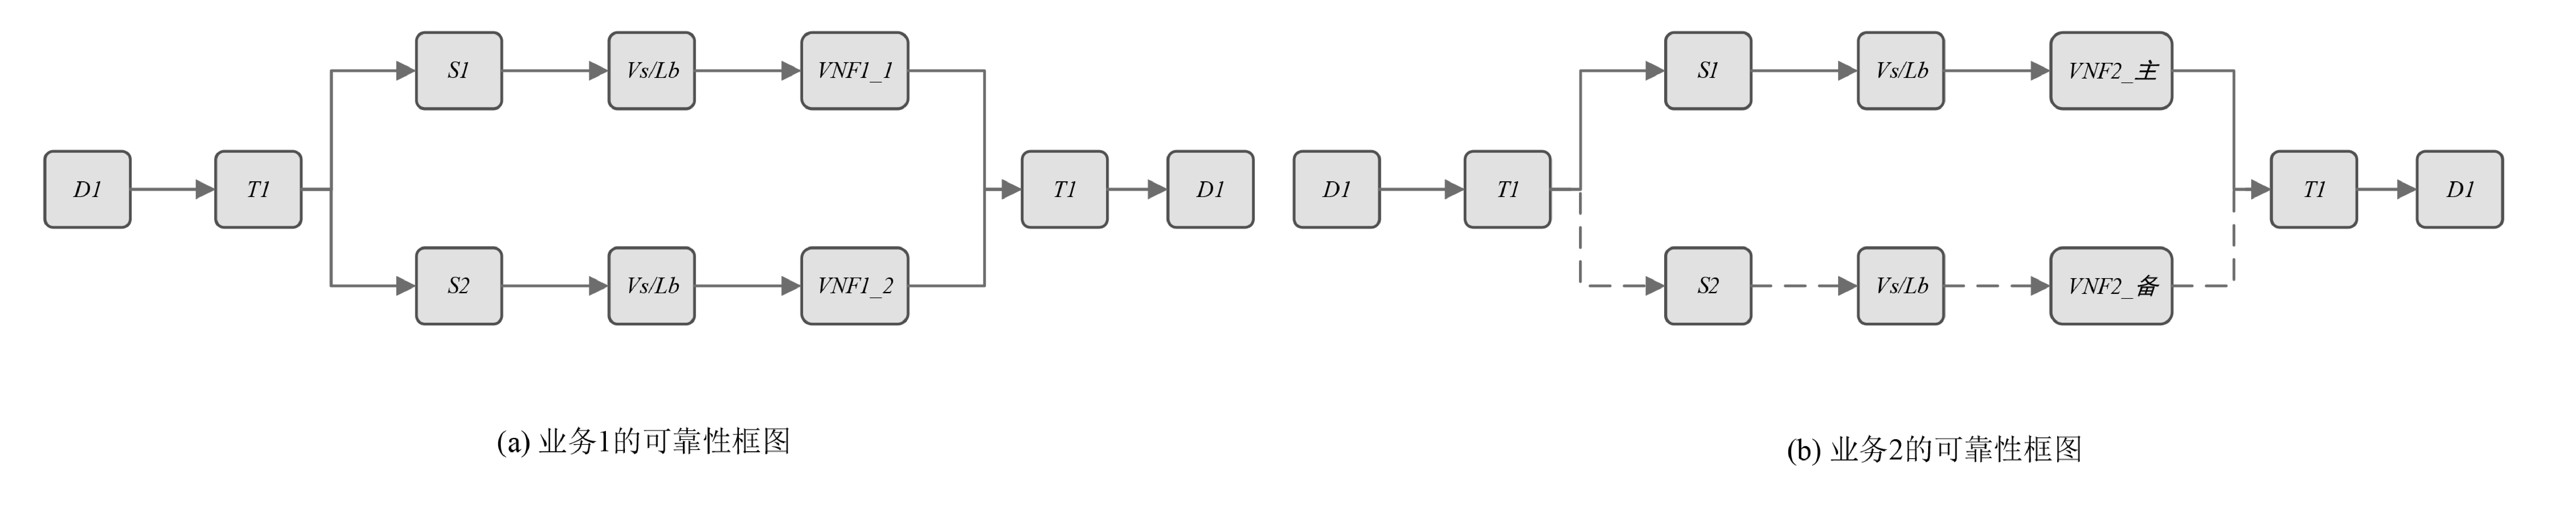
\includegraphics[width = 3in]{img/12.eps}
            \caption{Reliability block diagram analysis}
            \label{fig10}
        \end{center}
    \end{figure}

    At this time, the reliability of the two services can be expressed as:

    \begin{eqnarray}
        R_{app_1}&=& R_{D_1}* R_{T_1} * (1-(1-R_{S_1}*R_{Vs}*R_{VNF1\_1}) \nonumber\\
        &    & *(1-R_{S_2}*R_{Vs}*R_{VNF1\_2}))\\
        R_{app_2}&=& R_{D_1} * R_{T_1} * (R_{S_1}*R_{Vs}*R_{VNF} \nonumber\\
        & & +(1-R_{S_1}*R_{Vs}*R_{VNF2\_M})*p_s*R_{S_2} \nonumber\\
        & &*R_{Vs}*R_{VNF2\_s} )
    \end{eqnarray}

    According to the case parameter settings, because it is difficult to dynamically represent the network link, the initial link of the service is first used to estimate the reliability of the service virtual link. At this time:
    \begin{eqnarray}
        R_{D_1} &=& R_{T_1} = R_{S_1} = R_{S_2} = \frac{50*365*24}{50*365*24+2} \nonumber\\
                &=& 0.9999954338108045 \\
        R_{Vs/Lb} &=& R_{VNF1\_1} = R_{VNF1\_2} = R_{VNF2\_M} = R_{VNF2\_S}     \nonumber\\
                  &=& \frac{2*365*24}{2*365*24+(0.1*2+0.9*(10/60)))} \nonumber\\
                  &=& 0.9999800232301296
    \end{eqnarray}

%    \begin{equation}
%        \left\{ {\begin{array}{*{20}{c}}
%                     R_{D_1} = R_{T_1} = R_{S_1} = R_{S_2} = \frac{50*365*24}{50*365*24+2} \\=0.9999954338108045     \\
%                     R_{Vs/Lb} = R_{VNF1\_1} = R_{VNF1\_2} = R_{VNF2\_M} = R_{VNF2\_S}     \\= \frac{2*365*24}{2*365*24+2}=0.9998858577787924
%        \end{array}} \right.
%    \end{equation}

    With the switching probability $p_s = 0.9$, the reliability of the two services can be obtained as:

    \begin{equation}
        R_{app_1} = 0.9999908667951362, R_{app_2} = 0.9999879560119541
    \end{equation}

    The two service reliability values calculated using the network evolution method proposed in the article are shown in the table (calculation period $T=200 years$):

    \begin{table}[!t]
        \renewcommand{\arraystretch}{1.3}
        \caption{Case parameter setting}
        \label{tab11}
        \centering
        \begin{tabular}{|c|c|c|c|c|c|}
            \hline
            N                & 10       & 50       & 100      & 200      & 500      \\
            \hline
            App1 Reliability & 0.999980 & 0.999989 & 0.999990 & 0.999990 & 0.999990 \\
            App2 Reliability & 0.999913 & 0.999941 & 0.999933 & 0.99994  & 0.99994  \\
            \hline
        \end{tabular}
    \end{table}

    \subsection{Algorithm convergence analysis}
    Since some parameters of the factors affecting the network evolution conditions in this article are randomly distributed, we take the average value to estimate the subsequent business reliability. According to the central limit law, the mathematical expectation $R_i$ and variance $\delta^2$ of the independent random variable business reliability $\bar{R_i}$ for $n$ simulations, then:

    \begin{equation}
        \mathop {\lim }\limits_{n \to \infty } P\left\{ {\frac{{\overline {{R_i}}  - {R_i}}}{{\sigma  - \sqrt n }} < {t_\alpha }} \right\}{\rm{ = }}\int_{{\rm{ - }}\infty }^{{t_\alpha }} {\frac{1}{{\sqrt {2\pi } }}} {e^{{{ - {t^2}} \mathord{\left/
                {\vphantom {{ - {t^2}} 2}} \right.
            \kern-\nulldelimiterspace} 2}}}dt = \Phi \left( {{t_\alpha }} \right)
    \end{equation}

    At this time, the absolute error of the simulation is:

    \begin{equation}
        \varepsilon  = \frac{{{\lambda _\alpha }\sigma }}{{\sqrt n }}
    \end{equation}

    We first analyzed the average availability and simulation errors of the selected five businesses (App6, App11, App16, App26, and App31). Taking T=50 years and a confidence level of 95\%, the changes in the business average and the simulation absolute error with the number of simulations are plotted, and the error threshold is $10^(-4)$. It can be seen that for these 5 services, as the number of simulations increases, the mean value gradually converges; when the number of simulations is 6, 18, 53, 73, and 77, the results can be satisfied with a confidence level of 95\%. Simulation accuracy requirements. It can be seen that the average business reliability calculated by this algorithm gradually converges as the number of calculations increases.

    \begin{figure}[!t]
        \begin{center}
            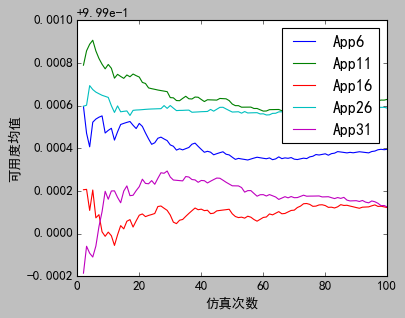
\includegraphics[width = 3in]{img/13.png}
            \caption{Variation of the mean availability with the number of simulations}
            \label{fig10}
        \end{center}
    \end{figure}

    \begin{figure}[!t]
        \begin{center}
            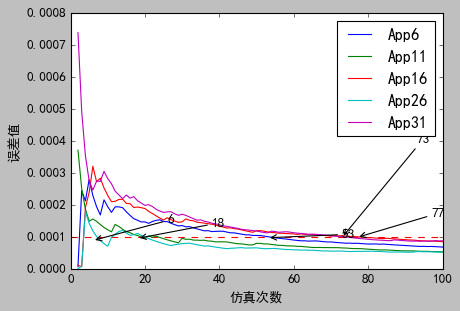
\includegraphics[width = 3in]{img/14.png}
            \caption{Variation of error with simulation times}
            \label{fig10}
        \end{center}
    \end{figure}

    \subsection{Influencing factors of Application reliability}
    Subsequently, we selected services with different logical path lengths and analyzed the relationship between the simulation error and the number of calculations and the single calculation cycle. It can be seen that as the simulation time increases, the simulation error of different services increases its simulation accuracy as the simulation cycle increases. Will improve. At the same time, comparing the three services, it can be seen that the convergence speed of the calculation results is not that the longer the business logic path, the faster the convergence. The two VNFs in App20 are both active and standby VNFs, so the convergence is the slowest; App60 contains two host-based VNFs, so the convergence speed is relatively fast; App15 includes a 2-way service, so although the logical path is shorter  , But the convergence speed is more balanced.


    \begin{figure}[!t]
        \begin{center}
            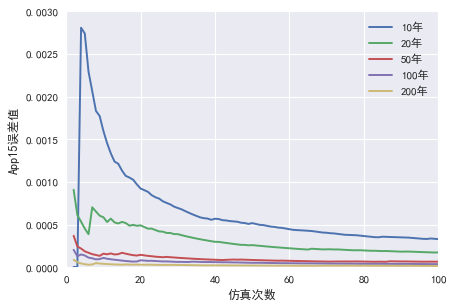
\includegraphics[width = 3in]{img/15.png}
            \caption{When the service (App15) uses 1 VNF, the relationship between the error and the number of calculations and the single calculation cycle}
            \label{fig10}
        \end{center}
    \end{figure}

    \begin{figure}[!t]
        \begin{center}
            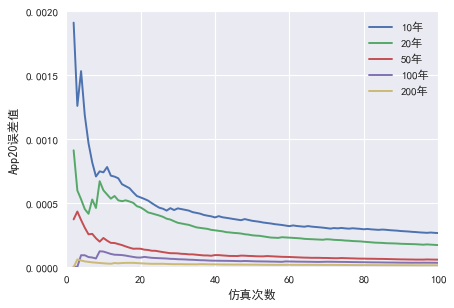
\includegraphics[width = 3in]{img/16.png}
            \caption{When the service (App20) uses 2 VNFs, the relationship between the error and the number of calculations and the single calculation cycle}
            \label{fig10}
        \end{center}
    \end{figure}

    \begin{figure}[!t]
        \begin{center}
            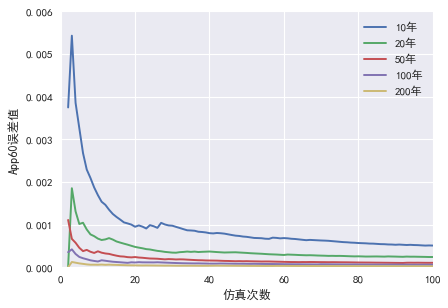
\includegraphics[width = 3in]{img/17.png}
            \caption{When the service (App60) uses 3 VNFs, the relationship between the error and the number of calculations and the single calculation cycle}
            \label{fig10}
        \end{center}
    \end{figure}

    Finally, we give the relationship between the calculation result of the whole network service reliability and the calculation cycle and the number of calculations, as shown in Table 6 and Table 7.

    \begin{table}[!t]
        \renewcommand{\arraystretch}{1.3}
        \caption{The calculation result and calculation time of the whole network service reliability when N=100, T=[10,20,50,100,200]}
        \label{tab11}
        \centering
        \begin{tabular}{|c|c|c|c|c|c|}
            \hline
            T(year) & 10       & 20       & 50       & 100      & 200      \\
            \hline
            Rel     & 0.996956 & 0.997944 & 0.999034 & 0.999503 & 0.999741 \\
            \hline
        \end{tabular}
    \end{table}

    \begin{table}[!t]
        \renewcommand{\arraystretch}{1.3}
        \caption{Reliability calculation results and calculation time of the entire network when T=200 and N=[10,50,100]}
        \label{tab11}
        \centering
        \begin{tabular}{|c|c|c|c|}
            \hline
            N   & 10       & 50       & 100      \\
            \hline
            Rel & 0.999725 & 0.999743 & 0.999743 \\
            \hline
        \end{tabular}
    \end{table}


% An example of a floating figure using the graphicx package.
% Note that \label must occur AFTER (or within) \caption.
% For figures, \caption should occur after the \includegraphics.
% Note that IEEEtran v1.7 and later has special internal code that
% is designed to preserve the operation of \label within \caption
% even when the captionsoff option is in effect. However, because
% of issues like this, it may be the safest practice to put all your
% \label just after \caption rather than within \caption{}.
%
% Reminder: the "draftcls" or "draftclsnofoot", not "draft", class
% option should be used if it is desired that the figures are to be
% displayed while in draft mode.
%
%\begin{figure}[!t]
%\centering
%\includegraphics[width=2.5in]{myfigure}
% where an .eps filename suffix will be assumed under latex, 
% and a .pdf suffix will be assumed for pdflatex; or what has been declared
% via \DeclareGraphicsExtensions.
%\caption{Simulation results for the network.}
%\label{fig_sim}
%\end{figure}

% Note that the IEEE typically puts floats only at the top, even when this
% results in a large percentage of a column being occupied by floats.


% An example of a double column floating figure using two subfigures.
% (The subfig.sty package must be loaded for this to work.)
% The subfigure \label commands are set within each subfloat command,
% and the \label for the overall figure must come after \caption.
% \hfil is used as a separator to get equal spacing.
% Watch out that the combined width of all the subfigures on a 
% line do not exceed the text width or a line break will occur.
%
%\begin{figure*}[!t]
%\centering
%\subfloat[Case I]{\includegraphics[width=2.5in]{box}%
%\label{fig_first_case}}
%\hfil
%\subfloat[Case II]{\includegraphics[width=2.5in]{box}%
%\label{fig_second_case}}
%\caption{Simulation results for the network.}
%\label{fig_sim}
%\end{figure*}
%
% Note that often IEEE papers with subfigures do not employ subfigure
% captions (using the optional argument to \subfloat[]), but instead will
% reference/describe all of them (a), (b), etc., within the main caption.
% Be aware that for subfig.sty to generate the (a), (b), etc., subfigure
% labels, the optional argument to \subfloat must be present. If a
% subcaption is not desired, just leave its contents blank,
% e.g., \subfloat[].


% An example of a floating table. Note that, for IEEE style tables, the
% \caption command should come BEFORE the table and, given that table
% captions serve much like titles, are usually capitalized except for words
% such as a, an, and, as, at, but, by, for, in, nor, of, on, or, the, to
% and up, which are usually not capitalized unless they are the first or
% last word of the caption. Table text will default to \footnotesize as
% the IEEE normally uses this smaller font for tables.
% The \label must come after \caption as always.
%
%\begin{table}[!t]
%% increase table row spacing, adjust to taste
%\renewcommand{\arraystretch}{1.3}
% if using array.sty, it might be a good idea to tweak the value of
% \extrarowheight as needed to properly center the text within the cells
%\caption{An Example of a Table}
%\label{table_example}
%\centering
%% Some packages, such as MDW tools, offer better commands for making tables
%% than the plain LaTeX2e tabular which is used here.
%\begin{tabular}{|c||c|}
%\hline
%One & Two\\
%\hline
%Three & Four\\
%\hline
%\end{tabular}
%\end{table}


% Note that the IEEE does not put floats in the very first column
% - or typically anywhere on the first page for that matter. Also,
% in-text middle ("here") positioning is typically not used, but it
% is allowed and encouraged for Computer Society conferences (but
% not Computer Society journals). Most IEEE journals/conferences use
% top floats exclusively. 
% Note that, LaTeX2e, unlike IEEE journals/conferences, places
% footnotes above bottom floats. This can be corrected via the
% \fnbelowfloat command of the stfloats package.


    \section{Conclusion}
    This paper proposes a reliability evaluation model of cloud virtualization based on network evolution. The model includes three parts: network evolution object, network evolution condition and network evolution rule. In the network evolution object modeling part, we established the network infrastructure layer (network nodes and edges) and network business layer (VNF and business) models. In the part of the network evolution condition model, we give out how to generate the relevant algorithms of component state changes over time according to the relevant parameters of the network component. In the part of network evolution rules, we clarified that after the status of each component changes, combined with the current status of the network to affect the status of each service in the network, we finally put forward the reliability evaluation algorithm of the single service and the whole network service of this model. The case verification results show that when the case-related design is simplified, the business reliability results obtained by us and the RBD algorithm are basically the same, and the calculation results of the algorithm converge. On this basis, we calculated and analyzed the service reliability on a large network of 128 servers carrying 100 services, and found that the service reliability is related to the length of the service logic path and the service protection strategy.


% if have a single appendix:
%\appendix[Proof of the Zonklar Equations]
% or
%\appendix  % for no appendix heading
% do not use \section anymore after \appendix, only \section*
% is possibly needed

% use appendices with more than one appendix
% then use \section to start each appendix
% you must declare a \section before using any
% \subsection or using \label (\appendices by itself
% starts a section numbered zero.)
%WW

%
%\appendices
%\section{Proof of the First Zonklar Equation}
%Appendix one text goes here.
%
%% you can choose not to have a title for an appendix
%% if you want by leaving the argument blank
%\section{}
%Appendix two text goes here.
%
%
%% use section* for acknowledgment

    \section*{Acknowledgment}
    The authors would like to thank the National Natural Science Foundation of China (No. 61872018).


% Can use something like this to put references on a page
% by themselves when using endfloat and the captionsoff option.
    \ifCLASSOPTIONcaptionsoff
    \newpage
    \fi


% trigger a \newpage just before the given reference
% number - used to balance the columns on the last page
% adjust value as needed - may need to be readjusted if
% the document is modified later
%\IEEEtriggeratref{8}
% The "triggered" command can be changed if desired:
%\IEEEtriggercmd{\enlargethispage{-5in}}

% references section

% can use a bibliography generated by BibTeX as a .bbl file
% BibTeX documentation can be easily obtained at:
% http://mirror.ctan.org/biblio/bibtex/contrib/doc/
% The IEEEtran BibTeX style support page is at:
% http://www.michaelshell.org/tex/ieeetran/bibtex/
%\bibliographystyle{IEEEtran}
% argument is your BibTeX string definitions and bibliography database(s)
%\bibliography{IEEEabrv,../bib/paper}
%
% <OR> manually copy in the resultant .bbl file
% set second argument of \begin to the number of references
% (used to reserve space for the reference number labels box)
%\begin{thebibliography}{1}
%
%\bibitem{IEEEhowto:kopka}
%H.~Kopka and P.~W. Daly, \emph{A Guide to \LaTeX}, 3rd~ed.\hskip 1em plus
%  0.5em minus 0.4em\relax Harlow, England: Addison-Wesley, 1999.
%
%\end{thebibliography}
    \bibliographystyle{ieeetr}
    \bibliography{ref}
% biography section
% 
% If you have an EPS/PDF photo (graphicx package needed) extra braces are
% needed around the contents of the optional argument to biography to prevent
% the LaTeX parser from getting confused when it sees the complicated
% \includegraphics command within an optional argument. (You could create
% your own custom macro containing the \includegraphics command to make things
% simpler here.)
%\begin{IEEEbiography}[{\includegraphics[width=1in,height=1.25in,clip,keepaspectratio]{mshell}}]{Michael Shell}
% or if you just want to reserve a space for a photo:

    \begin{IEEEbiography}{Juxing Zhu}
        Biography text here.
    \end{IEEEbiography}

    \begin{IEEEbiography}{Ning Huang}
        Biography text here.
    \end{IEEEbiography}

    \begin{IEEEbiography}{Sitong Caihuang}
        Biography text here.
    \end{IEEEbiography}

    \begin{IEEEbiography}{Junliang Wang}
        Biography text here.
    \end{IEEEbiography}
% if you will not have a photo at all:
%\begin{IEEEbiographynophoto}{John Doe}
%Biography text here.
%\end{IEEEbiographynophoto}

% insert where needed to balance the two columns on the last page with
% biographies
%\newpage
%
%\begin{IEEEbiographynophoto}{Jane Doe}
%Biography text here.
%\end{IEEEbiographynophoto}

% You can push biographies down or up by placing
% a \vfill before or after them. The appropriate
% use of \vfill depends on what kind of text is
% on the last page and whether or not the columns
% are being equalized.

%\vfill

% Can be used to pull up biographies so that the bottom of the last one
% is flush with the other column.
%\enlargethispage{-5in}


% that's all folks
\end{document}


